\documentclass[modern]{aastex63}
%\usepackage[bookmarks,bookmarksopen,colorlinks,linkcolor={blue},
%  citecolor={blue},urlcolor={blue}]{hyperref}
\hypersetup{linkcolor=blue,citecolor=blue,filecolor=blue,urlcolor=blue}
\usepackage{amsmath}
%\usepackage{natbib}
%\usepackage{color}
%\usepackage[x11names]{xcolor}
%%\usepackage{geometry}
%%\usepackage{pdflscape}
%\usepackage{graphics}
%\usepackage{enumerate}
%\usepackage{setspace}
%%\usepackage{siunitx}
\newcommand\gaia{\emph{Gaia}}
\newcommand\kepler{\emph{Kepler}}
\newcommand\ktwo{\emph{K2}}
\newcommand\tess{\emph{TESS}}
\newcommand\teff{$T_{\text{eff}}$}
\newcommand\logg{$\log{g}$}

\defcitealias{fulton18}{FP18}

\shortauthors{Cloutier et al.}
\shorttitle{The radius valley around low mass stars}

%% Nature astronomy article restrictions
%% 150 word abstract
%% 90 title characters
%% main text: 3000-3500 words
%% 6-8 figures+tables
%% <= 50 references in the main text
%% 500 words in the introduction (no header)
%% concise findings in the section "Results"
%% 1-2 paragraphs in the section "Discussion"


\begin{document}
\title{Evolution of the Radius Valley Around Low Mass Dwarf Stars with \emph{KEPLER} and \ktwo{}}

\correspondingauthor{Ryan Cloutier}
\email{cloutier@cfa.harvard.edu}
\author[0000-0001-5383-9393]{Ryan Cloutier}
\affiliation{Center for Astrophysics $|$ Harvard \& Smithsonian,
  60 Garden Street, Cambridge, MA, 02138, USA}
\affiliation{Dept. of Astronomy \& Astrophysics, University
of Toronto, 50 St. George Street, Toronto, ON, M5S 3H4, Canada}

\begin{abstract}  %% 150 words max
  Recent observational studies refining the planet radii around Sun-like stars revealed a gap
  in the occurrence-rate of close-in planet sizes. Resolving the so-called radius valley around low
  mass stars provides valuable constraints on the physical mechanisms sculpting the valley and so far
  are largely limited by relatively poor counting statistics. Here we calculate the occurrence-rate
  of small close-in planets around low mass stars from the primary \kepler{} and \ktwo{} missions.
  The radius
  valley is clearly resolved in the maximum-likelihood occurrence-rate although the gap is not
  completely void of planets, a feature whose prominence increases with decreasing stellar mass. In
  agreement with competing models of photoevaporation and core-powered mass-loss, we show that the
  valley location evolves to smaller planet radii with decreasing stellar mass. Robust inferences
  regarding the valley's dominant formation pathway will require $\mathcal{O}{(N)}$ additional
  confirmed planets which are expected to be uncovered by \tess{} within its extended mission.
\end{abstract}


\section{Introduction}
NASA's \kepler{} space telescope has discovered thousands of exoplanets over its lifetime and
consequently enabled robust investigations of the occurrence rate of planets within our galaxy.
%One striking outcome of such studies was that the so-called super-Earths and sub-Neptunes---whose
%radii span sizes intermediate between those of the Earth and Neptune---represent the most commmon
%type of planet around Sun-like stars and early M dwarfs alike
\citep[e.g.][]{youdin11,howard12,dressing13,fressin13,petigura13b,morton14,dressing15a}.
Furthermore, mass measurements of many of these transiting planets via transit-timing variations
or precision radial velocity follow-up campaigns revealed that the majority of planets
smaller than $\sim 1.6$ R$_{\oplus}$ are consistent with having bulk terrestrial compositions
\citep[e.g.][]{weiss14,dressing15b,rogers15}.
%Early investigations of the \kepler{} planet population noted that small planets are 
%preferentially found at short orbital periods where there is also a significant dearth of
%Neptune-sized planets \citep{benitezllambay11,beauge13,mazeh16}, commonly known as the Neptunian
%desert. Although the apparent dearth of small planets at long orbital periods is a clear artifact 
%of poor detection completeness, the lack of hot Neptunes is not.
Early studies of the \kepler{} population hinted at the distribution of planet radii at small orbital separations
featuring a bimodality \citep[e.g.][]{owen13}---commonly referred to as the radius valley---that
is thought to represent two populations of predominantly
rocky super-Earths plus inflated sub-Neptunes at slightly longer orbital periods
that have retained significant H/He envelopes.

Consequently, numerous studies of planet formation/evolution sought to explain the
apparent bimodality in the distribution of close-in planetary radii. One such proposed mechanism is
that of photoevaporation wherein the gaseous envelopes of small close-in planets may be stripped by
X-ray and extreme ultraviolet (XUV) radiation from their host stars during the first $\sim 100$ Myrs
of the planet's lifetime %\citep{jackson12}.
%thus leaving behind a population of bare (likely) rocky cores plus a population of inflated sub-Neptunes 
\citep{owen13,jin14,lopez14,chen16,lopez16,owen17,jin18}. Another possible explanation
invokes gas-poor formation wherein gas accretion is delayed by dynamical fraction whilst the
protoplanet is still embedded within the protoplanetary disk until a point at which the gaseous disk
has almost completely dissipated after just a few Myrs \citep{lee14,lee16}. More recently,
the radius valley may also be explained by core-powered mass loss wherein the
luminosity from a planetary core's primordial energy reservoir from formation drives atmospheric escape
over Gyr timescales \citep{ginzburg18,gupta19a,gupta19b}.

Observational tests of the aforementioned theoretical frameworks have become feasible in recent years as a result 
of the precise refinement of measured planet radii following improved stellar host characterization via  
spectroscopy, asteroseismology, and \gaia{} parallaxes
\citep[e.g.][]{fulton17,vaneylen18,fulton18,martinez19}. These studies clearly resolved the radius valley 
among small close-in planets around Sun-like stars. They also observed a variety of trends in either
the raw or in the completeness-corrected (i.e. the occurrence rate) distributions of close-in planets. Firstly,
the location of the radius valley around FGK stars is period-dependent with slope
$\mathrm{d}\log{r_p} / \mathrm{d}\log{P} \sim -0.1$ \citep{vaneylen18,martinez19}, a result that is consistent
with both photoevaporation and core-powered mass loss models but is inconsistent with the late formation of
terrestrial planets in a gas-poor environment. Secondly, the feature locations (i.e. the weighted
average radius of the peaks and valley) appear to exist at smaller planet radii with decreasing stellar
mass \citep{fulton18,wu19}.

In this study, we extend the investigation of close-in planets to systems hosted by
low mass dwarf stars later than mid-K. The known planet population in this stellar mass regime features
nearly ten times fewer planets than around Sun-like stars thus making the detection of the radius
valley around low mass stars more difficult and at a lower signal-to-noise. This fact is clearly evidenced in
the empirical \kepler{} planet population for which the radius valley around Sun-like stars (\teff{}
$\in [4700,6500]$ K) is clearly evident whereas any valley in the planet population around low mass stars
(\teff{} $< 4700$ K) is not easily discernible by-eye (Fig.~\ref{fig:berger}).
Our study leverages the precise stellar parallaxes from the \gaia{} DR2 \citep{lindegren18}
for low mass stars obseved by \kepler{} and \ktwo{} to refine the stellar parameters and compute precise
occurrence rates of close-in planets with the goal of resolving the radius valley and accurately measuring the
locations of the radius valley features and their uncertainties. Although it is unlikely that a single physical
mechanism is responsible for sculpting the radius valley, investigation the evolution of the valley features with
stellar mass can allude to which process---if any---dominates the evolution of close-in planets.

\begin{figure}
  \centering
  %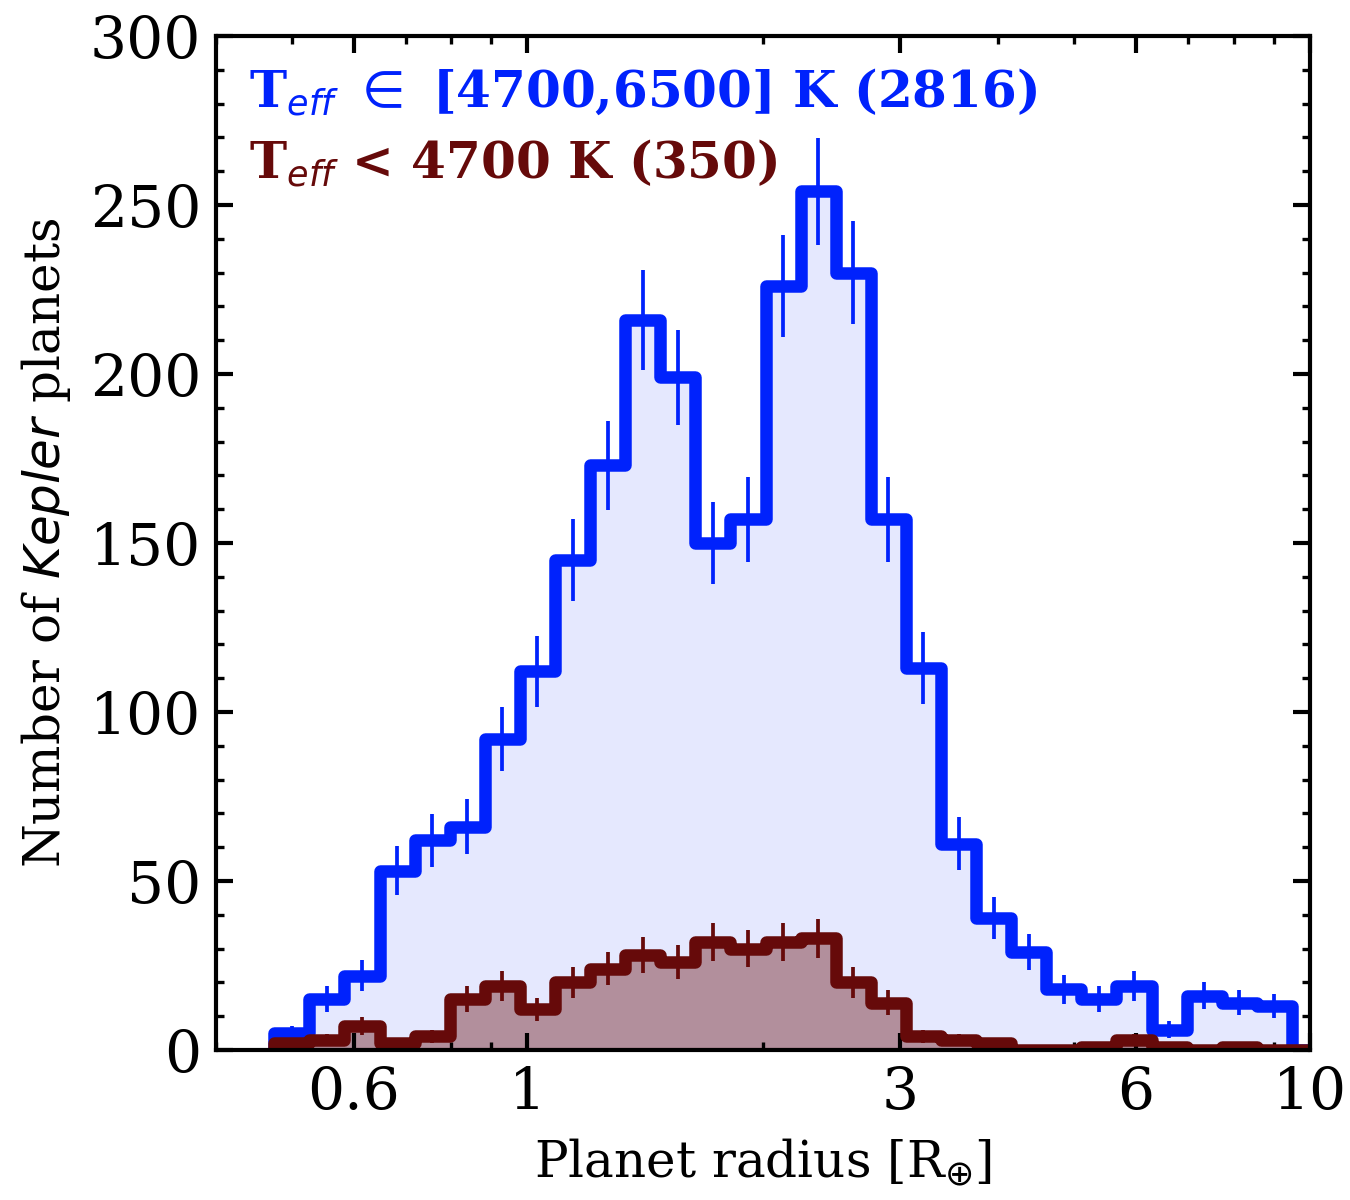
\includegraphics[width=0.98\hsize]{figures_tmp/Bergerplanethist.png}
  \caption{Empirical distributions of \kepler{} planet radii. Histograms of \kepler{} planet radii
    from \cite{berger18} for planets with host stellar effective temperatures \teff{} $\in [4700,6500]$ K
    (\emph{blue}) or \teff{} $<4700$ K (\emph{red}). The former subset of 2816 planets corresponds to the
    effective temperature range considered in the CKS \citep{fulton17}. The radius valley is clearly resolved
    in the empirical distribution of this sample (i.e. without completeness corrections). A similar bimodal
    structure is not resolved in the empirical disitribution of the latter subset of 350 planets around cooler
    stars.}
  \label{fig:berger}
\end{figure}

%In Sect.~\ref{sect:stars} we present our stellar sample from \kepler{} and \ktwo{.}
%In Sect.~\ref{sect:planets} we compile our sample of confirmed planets which we supplement with a
%suite of \ktwo{} planet candidates to improve the counting statistics.
%In Sect.~\ref{sect:completeness}
%we derive the transiting planet detection completeness from each mission and use those results to calculate
%the occurrence rate of small close-in planets and resolve the radius valley in Sect.~\ref{sect:occurrence}.
%Our results as a function stellar mass are compared to
%predictions from models of photoevaporation and core-powered mass loss in Sect.~\ref{sect:models}. We conclude 
%with a discussion of our results and its implications in Sect.~\ref{sect:conclusion}.


%\section{Sample of Low Mass Dwarf Stars from Kepler and K2} \label{sect:stars}
\section{Population of small close-in planets around low mass dwarf stars from Kepler and K2} \label{sect:planets}
The goal of this study is to extend measurements of the radius valley and its properties to planetary systems
hosted by low mass dwarf stars later than K3.5V \citep{pecaut13} with effective temperatures \teff{} $<4700$ K:
the lower limit of \teff{} considered by the California Kepler Survey where the radius valley was first revealed
\cite{fulton17}. Our stellar sample of interest therefore includes such stars from either \kepler{} or \ktwo{}
and up to maximum Kepler magnitudes of $K_p<X$ and $K_p<\mathbf{X}$ respectively.
The stellar radii are refined based on their spectroscopically-derived effective temperatures
\citep{gaidos16,mathur17,petigura17} and measured
luminosities which are derived from 2MASS $K_s$-band magnitudes \citep{cutri03} and \gaia{} DR2 stellar parallaxes
\citep{lindegren18} (see Methods). To investigate the evolution of the inherent planet population
with stellar mass, we employ a stellar mass-radius relation---applicable to K and M dwarfs---to derive stellar
masses from their measured radii \citep{boyajian12}.

We consider two planet populations separately. Our initial sample of transiting planets were retrieved from the
NASA Exoplanet Archive \citep{akeson13} on June 15, 2019 and only includes confirmed
planets with orbtial periods $P \in [0.5,100]$ days. By considering confirmed
planets only, we focus on the true empirical population of small close-in planets without being
contaminated by various astrophysical false positive scenarios that plague the planet candidates that are
excluded from our sample. The refined stellar parameters enable us to refine the planet radii by resampling
the stellar radius from its uncertainties and the scaled planet radius $r_p/R_s$ from its retreived 
point estimates to derive the planet radius. Similarly, we refine each planet's level of received insolation
given its orbital period plus its host star's \teff{,} $R_s$, and $M_s$. 
%The refined stellar radii derived in Sect.~\ref{sect:stars} enables us to derive more accurate and precise
%planet radii for the planets within our initial sample.
%We refine the planetary radii $r_p$ by first retrieving point estimates of each planet's scaled planetary radius
%$r_p/R_s$ which often include a median value 
%accompanied by the 16$^{\text{th}}$ and 84$^{\text{th}}$ percentiles. In cases for which the $r_p/R_s$ uncertainti%es
%are symmetric, we assume the $r_p/R_s$ posterior is Gaussian. For planets with asymmetric reported
%uncertainties, we fit the $r_p/R_s$ percentiles with a skew-normal random distribution using the
%\texttt{scipy.skewnorm python} class. We fit for the location, the scale, and the shape parameters of a
%skew-normal distrution whose percentiles are consistent with
%the reported $r_p/R_s$ point estimates for each planet. The refined planetary radii are then derived by sampling
%the $r_p/R_s$ distribution and the distribution of the refined host stellar radius. We then update our planet
%sample by only focusing on planets that are consistent with being between 0.5-4 R$_{\oplus}$.
%Similarly, given the distributions of the refined \teff{,} $M_s$, and $P$, we derive each planet's level of
%insolation as
%\begin{equation}
%  \frac{F}{F_{\oplus}} = \left( \frac{R_s}{R_{\odot}} \right)^2  \left( \frac{T_{\text{eff}}}{5777 \text{ K}} \right)^4 \left( \frac{a}{1 \text{ AU}} \right)^{-2} 
%\end{equation}
%\noindent where $a$ is the planet's semimajor axis.
Our final sample of confirmed small close-in planets with $P\in [0.5,100]$ days and $r_p\in [0.5,4]$ R$_{\oplus}$
contains \textbf{262} \kepler{} and \textbf{47} \ktwo{} planets respectively (Fig.~\ref{fig:Ndet}).
%Our planet sample
%of \textbf{309} confirmed planets is depicted in
%Fig.~\ref{fig:Ndet} along with the planet properties being reported in Tables~\ref{table:planetsKep}
%and~\ref{table:planetsK2}.

%\capstartfalse
\begin{deluxetable*}{ccccccccc}
\tabletypesize{\small}
\tablecaption{Kepler confirmed planet parameters\label{table:planetsKep}}
\tablehead{KIC & Planet & $P$ & $F$ & $F$ upper limit & $F$ lower limit & $r_p$ & $r_p$ upper limit & $r_p$ lower limit \\
& name & [days] & [F$_{\oplus}$] & [F$_{\oplus}$] & [F$_{\oplus}$] & [R$_{\oplus}$] & [R$_{\oplus}$] & [R$_{\oplus}$]}
\startdata
2556650 & Kepler-1124 b & 2.85235 & 46.5 & 4.7 & 4.6 & 1.97 & 0.08 & 0.10 \\
2715135 & Kepler-753 b & 5.74771 & 40.2 & 4.6 & 4.5 & 1.89 & 0.30 & 0.12 \\
3234598 & Kepler-383 b & 12.90468 & 20.2 & 2.8 & 2.5 & 1.54 & 0.30 & 0.17 \\
3234598 & Kepler-383 c & 31.20122 & 6.2 & 0.8 & 0.8 & 1.49 & 0.34 & 0.22 \\
3426367 & Kepler-1308 b & 2.10434 & 55.3 & 5.6 & 5.1 & 0.89 & 0.03 & 0.14
%%3444588 & Kepler-787 b & 0.92831 & 455.5 & 59.4 & 51.4 & 1.34 & 0.09 & 0.08 \\
%%3546060 & Kepler-1110 b & 9.69311 & 38.1 & 8.3 & 7.2 & 2.44 & 0.51 & 0.20 \\
%%3554031 & Kepler-415 c & 8.70798 & 24.8 & 3.5 & 2.8 & 2.25 & 0.16 & 0.12 \\
%%3554031 & Kepler-415 b & 4.17634 & 66.3 & 8.3 & 8.0 & 1.38 & 0.11 & 0.11 \\
%%3642335 & Kepler-1410 b & 60.86610 & 0.8 & 0.1 & 0.1 & 1.38 & 0.11 & 0.11 \\
%%3728432 & Kepler-1526 b & 3.90863 & 94.2 & 20.1 & 16.8 & 1.94 & 0.17 & 0.14 \\
%%3733628 & Kepler-543 b & 13.89963 & 21.9 & 2.6 & 2.3 & 2.54 & 0.11 & 0.30 \\
%%3859079 & Kepler-786 b & 53.52927 & 3.8 & 0.4 & 0.4 & 2.30 & 0.12 & 0.14 \\
%%3966801 & Kepler-577 b & 25.69581 & 4.3 & 0.4 & 0.4 & 2.66 & 0.27 & 0.16 \\
%%4056616 & Kepler-1053 b & 2.41435 & 150.6 & 17.6 & 16.0 & 0.82 & 0.05 & 0.04 \\
%%4139816 & Kepler-235 b & 3.34022 & 57.7 & 6.1 & 5.7 & 2.50 & 0.25 & 0.25 \\
%%4139816 & Kepler-235 c & 7.82502 & 18.4 & 1.9 & 1.8 & 1.48 & 0.27 & 0.27 \\
%%4139816 & Kepler-235 d & 20.06036 & 5.3 & 0.5 & 0.5 & 2.42 & 0.40 & 0.11 \\
%%4139816 & Kepler-235 e & 46.18420 & 1.7 & 0.2 & 0.2 & 2.25 & 0.11 & 0.11 \\
%%4249725 & Kepler-120 b & 6.31251 & 36.2 & 3.9 & 3.6 & 2.55 & 0.10 & 0.07 \\
%%4249725 & Kepler-120 c & 12.79455 & 14.1 & 1.5 & 1.4 & 2.04 & 0.07 & 0.07 \\
%%4263293 & Kepler-331 d & 32.13400 & 5.0 & 1.0 & 0.9 & 2.71 & 0.23 & 0.23 \\
%%4263293 & Kepler-331 b & 8.45747 & 29.6 & 6.5 & 5.5 & 2.78 & 0.21 & 0.21 \\
%%4263293 & Kepler-331 c & 17.28117 & 11.6 & 2.7 & 2.0 & 3.02 & 0.23 & 0.23 \\
%%4633570 & Kepler-158 b & 16.70921 & 13.4 & 1.5 & 1.4 & 2.18 & 0.10 & 0.36 \\
%%4633570 & Kepler-158 c & 28.55158 & 6.5 & 0.7 & 0.8 & 1.90 & 0.33 & 0.33 \\
%%4725681 & Kepler-236 b & 8.29562 & 14.0 & 1.5 & 1.3 & 2.13 & 0.41 & 0.41 \\
%%4725681 & Kepler-236 c & 23.96794 & 3.4 & 0.4 & 0.3 & 2.10 & 0.07 & 0.12 \\
%%4736569 & Kepler-1042 b & 10.13201 & 25.1 & 5.8 & 4.6 & 1.69 & 0.12 & 0.13 \\
%%4832837 & Kepler-621 b & 2.62812 & 69.8 & 35.4 & 22.5 & 1.82 & 0.31 & 0.30 \\
%%4852528 & Kepler-80 d & 3.07215 & 145.6 & 17.3 & 17.1 & 1.56 & 0.08 & 0.08 \\
%%4852528 & Kepler-80 c & 9.52164 & 32.0 & 4.2 & 3.5 & 2.59 & 0.12 & 0.12 \\
%%4852528 & Kepler-80 e & 4.64538 & 84.0 & 11.0 & 9.5 & 1.60 & 0.08 & 0.08 \\
%%4852528 & Kepler-80 f & 0.98679 & 662.4 & 84.9 & 75.9 & 1.43 & 0.07 & 0.07 \\
%%4852528 & Kepler-80 b & 7.05353 & 48.3 & 6.4 & 5.3 & 2.59 & 0.12 & 0.11 \\
%%4913852 & Kepler-691 b & 8.11437 & 12.2 & 1.3 & 1.2 & 2.32 & 0.38 & 0.12 \\
%%4917596 & Kepler-1032 b & 3.29011 & 138.4 & 30.4 & 29.5 & 2.00 & 0.20 & 0.17 \\
%%5080636 & Kepler-974 b & 4.19450 & 28.1 & 2.9 & 2.7 & 1.64 & 0.06 & 0.24 \\
%%5175986 & Kepler-1320 b & 0.86839 & 752.8 & 156.1 & 144.9 & 1.32 & 0.12 & 0.11 \\
%%5184911 & Kepler-1324 b & 4.11586 & 106.4 & 22.7 & 19.4 & 1.55 & 0.39 & 0.25 \\
%%5185897 & Kepler-398 c & 11.41942 & 20.3 & 2.4 & 2.2 & 1.02 & 0.21 & 0.21 \\
%%5185897 & Kepler-398 b & 4.08141 & 80.0 & 9.3 & 8.9 & 1.03 & 0.06 & 0.18 \\
%%5185897 & Kepler-398 d & 6.83441 & 40.4 & 4.7 & 4.8 & 1.04 & 0.19 & 0.19 \\
%%5209845 & Kepler-1378 b & 11.95402 & 15.5 & 3.3 & 2.9 & 1.91 & 0.67 & 0.26 \\
%%5269467 & Kepler-925 b & 33.86778 & 5.6 & 1.2 & 1.0 & 2.33 & 0.46 & 0.34 \\
%%5340644 & Kepler-580 b & 8.22241 & 23.3 & 3.2 & 2.6 & 2.34 & 0.12 & 0.11 \\
%%5364071 & Kepler-49 e & 18.59612 & 5.4 & 0.6 & 0.5 & 1.77 & 0.08 & 0.08 \\
%%5364071 & Kepler-49 c & 10.91274 & 11.0 & 1.1 & 1.1 & 2.47 & 0.23 & 0.15 \\
%%5364071 & Kepler-49 b & 7.20386 & 19.2 & 2.1 & 1.9 & 2.61 & 0.08 & 0.08 \\
%%5364071 & Kepler-49 d & 2.57657 & 75.5 & 7.8 & 7.5 & 1.82 & 0.06 & 0.06 \\
%%5371776 & Kepler-304 b & 3.29570 & 157.5 & 18.5 & 16.6 & 2.68 & 0.15 & 0.14 \\
%%5371776 & Kepler-304 e & 1.49914 & 452.4 & 56.2 & 45.6 & 1.04 & 0.07 & 0.07 \\
%%5371776 & Kepler-304 d & 9.65349 & 37.9 & 4.2 & 4.0 & 2.29 & 0.13 & 0.13 \\
%%5371776 & Kepler-304 c & 5.31595 & 83.6 & 8.9 & 9.4 & 2.22 & 0.28 & 0.28 \\
%%5526527 & Kepler-970 b & 16.73648 & 10.8 & 1.3 & 1.2 & 2.74 & 0.76 & 0.62 \\
%%5531576 & Kepler-240 b & 4.14452 & 146.3 & 23.5 & 21.4 & 1.45 & 0.11 & 0.11 \\
%%5531576 & Kepler-240 c & 7.95355 & 60.9 & 8.6 & 8.6 & 2.19 & 0.13 & 0.13 \\
%%5617854 & Kepler-901 b & 3.51749 & 64.6 & 8.2 & 7.1 & 1.54 & 0.07 & 0.17 \\
%%5640085 & Kepler-159 b & 10.13959 & 28.2 & 3.2 & 2.9 & 2.22 & 0.11 & 0.10 \\
%%5640085 & Kepler-159 c & 43.58594 & 4.0 & 0.5 & 0.4 & 2.70 & 0.14 & 0.14 \\
%%5686174 & Kepler-622 b & 14.28228 & 11.5 & 1.3 & 1.2 & 2.09 & 0.11 & 0.09 \\
%%5688790 & Kepler-1439 b & 8.07394 & 8.6 & 0.9 & 0.8 & 1.77 & 0.09 & 0.39 \\
%%5706966 & Kepler-333 c & 24.08842 & 6.3 & 0.8 & 0.7 & 1.34 & 0.09 & 0.09 \\
%%5706966 & Kepler-333 b & 12.55111 & 15.0 & 1.9 & 1.7 & 1.55 & 0.39 & 0.09 \\
%%5794379 & Kepler-241 b & 12.71810 & 22.8 & 6.3 & 5.1 & 2.28 & 0.19 & 0.22 \\
%%5794379 & Kepler-241 c & 36.06588 & 5.7 & 1.4 & 1.2 & 2.63 & 0.22 & 0.24 \\
%%5868793 & Kepler-1582 b & 4.83809 & 4.3 & 0.4 & 0.4 & 0.85 & 0.07 & 0.06 \\
%%5940165 & Kepler-1062 b & 9.30414 & 30.0 & 6.3 & 5.0 & 1.85 & 0.14 & 0.19 \\
%%5980208 & Kepler-1331 b & 0.78916 & 523.6 & 120.1 & 87.0 & 0.90 & 0.07 & 0.08 \\
%%6020753 & Kepler-202 c & 16.28248 & 17.4 & 2.1 & 2.1 & 1.91 & 0.11 & 0.11 \\
%%6020753 & Kepler-202 b & 4.06943 & 111.5 & 12.6 & 12.5 & 1.55 & 0.09 & 0.07 \\
%%6026438 & Kepler-354 b & 5.47666 & 66.2 & 14.4 & 12.1 & 1.92 & 0.15 & 0.28 \\
%%6026438 & Kepler-354 d & 24.21020 & 9.2 & 2.0 & 1.6 & 1.43 & 0.15 & 0.15 \\
%%6026438 & Kepler-354 c & 16.93481 & 15.0 & 2.9 & 2.7 & 1.25 & 0.12 & 0.12 \\
%%6063220 & Kepler-99 b & 4.60358 & 113.0 & 12.8 & 13.1 & 1.51 & 0.07 & 0.07 \\
%%6186964 & Kepler-1366 b & 2.16457 & 119.0 & 12.3 & 11.5 & 1.57 & 0.07 & 0.09 \\
%%6205897 & Kepler-1029 b & 4.41769 & 94.1 & 10.5 & 9.0 & 1.52 & 0.25 & 0.37 \\
%%6263593 & Kepler-1418 b & 22.47660 & 7.1 & 1.4 & 1.2 & 1.21 & 0.15 & 0.11 \\
%%6382217 & Kepler-353 c & 8.41100 & 14.8 & 1.6 & 1.6 & 2.13 & 0.06 & 0.38 \\
%%6382217 & Kepler-353 b & 5.79529 & 24.4 & 2.7 & 2.4 & 1.25 & 0.35 & 0.35 \\
%%6425957 & Kepler-205 c & 20.30653 & 6.4 & 0.8 & 0.7 & 1.82 & 0.17 & 0.17 \\
%%6425957 & Kepler-205 b & 2.75564 & 93.1 & 11.1 & 10.0 & 1.58 & 0.09 & 0.12 \\
%%6435936 & Kepler-705 b & 56.05608 & 0.8 & 0.1 & 0.1 & 2.21 & 0.11 & 0.09 \\
%%6436029 & Kepler-1359 b & 59.49690 & 2.7 & 0.4 & 0.3 & 2.29 & 0.12 & 0.18 \\
%%6444896 & Kepler-1649 b & 8.68911 & 0.7 & nan & nan & 0.49 & 0.06 & 0.06 \\
%%6497146 & Kepler-438 b & 35.23307 & 1.7 & 0.3 & 0.3 & 0.97 & 0.09 & 0.08 \\
%%6665512 & Kepler-1048 b & 6.92101 & 33.0 & 8.4 & 7.3 & 2.46 & 0.34 & 0.30 \\
%%6697756 & Kepler-1351 b & 0.91614 & 412.9 & 80.8 & 83.5 & 0.55 & 0.05 & 0.04 \\
%%6773862 & Kepler-988 b & 17.76077 & 5.7 & 0.6 & 0.5 & 2.37 & 0.34 & 0.14 \\
%%6921944 & Kepler-1105 b & 4.42157 & 51.8 & 6.0 & 5.7 & 1.83 & 0.08 & 0.34 \\
%%6949607 & Kepler-28 c & 8.98582 & 32.9 & 4.1 & 3.7 & 1.88 & 0.10 & 0.10 \\
%%6949607 & Kepler-28 b & 5.91227 & 57.3 & 7.5 & 6.4 & 1.97 & 0.10 & 0.09 \\
%%6960913 & Kepler-61 b & 59.87803 & 1.5 & 0.1 & 0.1 & 2.48 & 0.11 & 0.08 \\
%%7021681 & Kepler-505 b & 27.52195 & 3.1 & 0.3 & 0.3 & 3.11 & 0.09 & 0.11 \\
%%7033233 & Kepler-1197 b & 2.03232 & 274.1 & 33.5 & 29.8 & 1.12 & 0.11 & 0.05 \\
%%7094486 & Kepler-1009 b & 11.35011 & 9.2 & 0.9 & 0.8 & 2.38 & 0.12 & 0.09 \\
%%7287995 & Kepler-81 d & 20.83763 & 7.3 & 0.8 & 0.8 & 1.44 & 0.36 & 0.36 \\
%%7287995 & Kepler-81 c & 12.03987 & 15.2 & 1.9 & 1.5 & 2.22 & 0.11 & 0.11 \\
%%7287995 & Kepler-81 b & 5.95490 & 38.6 & 4.3 & 4.1 & 2.37 & 0.11 & 0.12 \\
%%7304449 & Kepler-1650 b & 1.53818 & 43.1 & 4.5 & 4.3 & 1.34 & 0.08 & 0.26 \\
%%7350067 & Kepler-1646 b & 4.48559 & 9.1 & 1.5 & 1.3 & 1.84 & 0.09 & 0.14 \\
%%7439316 & Kepler-866 b & 2.61703 & 199.7 & 42.6 & 37.2 & 1.44 & 0.13 & 0.11 \\
%%7447200 & Kepler-210 b & 2.45324 & 102.7 & 10.4 & 9.2 & 3.00 & 0.18 & 0.18 \\
%%7455287 & Kepler-54 c & 12.07134 & 6.6 & 0.7 & 0.6 & 1.44 & 0.08 & 0.08 \\
%%7455287 & Kepler-54 d & 20.99588 & 3.1 & 0.3 & 0.3 & 1.46 & 0.07 & 0.07 \\
%%7455287 & Kepler-54 b & 8.01078 & 11.3 & 1.2 & 1.1 & 1.92 & 0.06 & 0.06 \\
%%7603200 & Kepler-138 b & 10.31282 & 9.5 & 1.1 & 0.9 & 0.63 & 0.03 & 0.03 \\
%%7603200 & Kepler-138 c & 13.78109 & 6.4 & 0.7 & 0.6 & 1.52 & 0.14 & 0.06 \\
%%7603200 & Kepler-138 d & 23.08902 & 3.2 & 0.3 & 0.3 & 1.32 & 0.05 & 0.05 \\
%%7676423 & Kepler-1430 b & 2.46050 & 203.6 & 55.6 & 47.1 & 1.04 & 0.12 & 0.11 \\
%%7802719 & Kepler-1157 b & 4.45743 & 81.1 & 17.3 & 14.0 & 0.93 & 0.09 & 0.07 \\
%%7826620 & Kepler-1579 b & 0.84991 & 376.6 & 110.2 & 86.1 & 0.56 & 0.06 & 0.07 \\
%%7870390 & Kepler-83 d & 5.16980 & 30.6 & 3.5 & 3.0 & 2.00 & 0.08 & 0.08 \\
%%7870390 & Kepler-83 b & 9.77045 & 13.1 & 1.4 & 1.3 & 2.69 & 0.10 & 0.08 \\
%%7870390 & Kepler-83 c & 20.09017 & 5.0 & 0.6 & 0.5 & 2.71 & 0.36 & 0.36 \\
%%7871954 & Kepler-303 c & 7.06117 & 22.4 & 2.3 & 2.3 & 1.49 & 0.18 & 0.18 \\
%%7871954 & Kepler-303 b & 1.93703 & 124.4 & 12.1 & 12.3 & 1.06 & 0.04 & 0.04 \\
%%7907423 & Kepler-249 d & 15.36846 & 3.9 & 0.4 & 0.4 & 1.38 & 0.06 & 0.06 \\
%%7907423 & Kepler-249 b & 3.30655 & 30.2 & 3.2 & 2.8 & 1.13 & 0.05 & 0.05 \\
%%7907423 & Kepler-249 c & 7.11373 & 10.9 & 1.2 & 1.1 & 1.45 & 0.05 & 0.06 \\
%%8009350 & Kepler-892 b & 13.75208 & 19.5 & 4.5 & 3.5 & 2.52 & 0.28 & 0.42 \\
%%8016691 & Kepler-1456 b & 18.13738 & 7.8 & 1.8 & 1.5 & 1.40 & 0.29 & 0.42 \\
%%8120608 & Kepler-186 e & 22.40778 & 3.1 & 0.3 & 0.3 & 1.40 & 0.06 & 0.06 \\
%%8120608 & Kepler-186 d & 13.34300 & 6.2 & 0.6 & 0.6 & 1.57 & 0.22 & 0.22 \\
%%8120608 & Kepler-186 c & 7.26731 & 13.8 & 1.4 & 1.3 & 1.39 & 0.05 & 0.04 \\
%%8120608 & Kepler-186 b & 3.88680 & 32.1 & 3.2 & 2.9 & 1.18 & 0.04 & 0.04 \\
%%8125580 & Kepler-749 b & 17.31712 & 19.0 & 3.7 & 3.5 & 3.21 & 0.70 & 0.30 \\
%%8150320 & Kepler-55 f & 10.19849 & 25.3 & 3.2 & 2.9 & 1.83 & 0.39 & 0.39 \\
%%8150320 & Kepler-55 e & 4.61749 & 72.9 & 9.1 & 8.4 & 1.70 & 0.22 & 0.22 \\
%%8150320 & Kepler-55 b & 27.95413 & 6.6 & 0.9 & 0.8 & 1.99 & 0.14 & 0.14 \\
%%8150320 & Kepler-55 c & 42.14061 & 3.8 & 0.5 & 0.4 & 1.94 & 0.21 & 0.18 \\
%%8150320 & Kepler-55 d & 2.21112 & 194.8 & 25.5 & 22.3 & 1.94 & 0.21 & 0.21 \\
%%8151055 & Kepler-1460 b & 29.96328 & 5.3 & 1.2 & 0.9 & 2.22 & 0.31 & 0.42 \\
%%8167996 & Kepler-327 c & 5.21230 & 24.5 & 2.6 & 2.3 & 1.24 & 0.05 & 0.05 \\
%%8167996 & Kepler-327 d & 13.96950 & 6.6 & 0.7 & 0.6 & 2.44 & 0.41 & 0.41 \\
%%8167996 & Kepler-327 b & 2.54956 & 64.0 & 6.5 & 5.8 & 1.33 & 0.06 & 0.04 \\
%%8183288 & Kepler-437 b & 66.65045 & 2.2 & 0.2 & 0.2 & 1.54 & 0.09 & 0.09 \\
%%8229458 & Kepler-1152 b & 1.64680 & 126.9 & 12.5 & 12.1 & 1.02 & 0.05 & 0.04 \\
%%8230616 & Kepler-316 b & 2.24049 & 148.0 & 18.0 & 17.8 & 1.45 & 0.06 & 0.10 \\
%%8230616 & Kepler-316 c & 6.82778 & 33.4 & 4.1 & 3.6 & 1.60 & 0.08 & 0.08 \\
%%8235924 & Kepler-1203 b & 0.58800 & 619.6 & 59.3 & 57.6 & 1.22 & 0.04 & 0.06 \\
%%8247771 & Kepler-1200 b & 1.11855 & 532.8 & 124.5 & 92.4 & 1.07 & 0.10 & 0.09 \\
%%8282651 & Kepler-1136 b & 2.36172 & 153.6 & 30.5 & 27.3 & 1.44 & 0.13 & 0.11 \\
%%8346392 & Kepler-777 b & 5.72813 & 30.6 & 3.0 & 3.0 & 1.62 & 0.08 & 0.08 \\
%%8351704 & Kepler-779 b & 7.09712 & 11.9 & 1.3 & 1.3 & 1.04 & 0.06 & 0.05 \\
%%8367644 & Kepler-993 b & 22.08552 & 3.9 & 0.4 & 0.4 & 3.48 & 0.58 & 0.30 \\
%%8424002 & Kepler-1512 b & 20.35972 & 1.5 & 0.7 & 0.6 & 0.79 & 0.12 & 0.17 \\
%%8463346 & Kepler-436 c & 16.79716 & 15.2 & 2.2 & 2.0 & 2.59 & 0.20 & 0.55 \\
%%8463346 & Kepler-436 b & 64.00197 & 2.6 & 0.4 & 0.3 & 2.34 & 0.51 & 0.51 \\
%%8505670 & Kepler-252 c & 10.84845 & 18.6 & 2.1 & 2.2 & 2.76 & 0.14 & 0.12 \\
%%8505670 & Kepler-252 b & 6.66833 & 35.8 & 4.1 & 3.8 & 1.39 & 0.54 & 0.54 \\
%%8544992 & Kepler-388 c & 13.29707 & 16.5 & 3.9 & 3.3 & 0.91 & 0.10 & 0.09 \\
%%8544992 & Kepler-388 b & 3.17323 & 110.0 & 25.0 & 21.8 & 0.89 & 0.09 & 0.09 \\
%%8547140 & Kepler-801 b & 11.41926 & 11.5 & 1.2 & 1.2 & 2.07 & 0.07 & 0.07 \\
%%8561063 & Kepler-42 b & 1.21377 & 22.6 & 2.5 & 2.3 & 0.91 & 0.03 & 0.12 \\
%%8561063 & Kepler-42 d & 1.86511 & 12.8 & 1.3 & 1.3 & 0.77 & 0.09 & 0.09 \\
%%8733898 & Kepler-446 d & 5.14892 & 4.9 & 0.5 & 0.4 & 1.14 & 0.23 & 0.23 \\
%%8733898 & Kepler-446 c & 3.03621 & 9.8 & 1.1 & 1.0 & 0.93 & 0.05 & 0.05 \\
%%8733898 & Kepler-446 b & 1.56541 & 23.6 & 2.4 & 2.3 & 1.15 & 0.06 & 0.04 \\
%%8826007 & Kepler-1450 b & 54.50915 & 2.7 & 0.7 & 0.5 & 2.33 & 0.21 & 0.60 \\
%%8845205 & Kepler-560 b & 18.47763 & 1.8 & 0.2 & 0.2 & 2.21 & 0.18 & 0.15 \\
%%8874090 & Kepler-834 b & 13.32389 & 9.0 & 1.0 & 0.9 & 1.97 & 0.10 & 0.08 \\
%%8890150 & Kepler-395 c & 34.98978 & 2.2 & 0.2 & 0.2 & 1.41 & 0.11 & 0.08 \\
%%8890150 & Kepler-395 b & 7.05429 & 18.8 & 2.0 & 1.7 & 1.24 & 0.11 & 0.11 \\
%%8978528 & Kepler-329 b & 7.41635 & 32.3 & 4.0 & 3.6 & 1.72 & 0.12 & 0.12 \\
%%8978528 & Kepler-329 c & 18.68484 & 9.4 & 1.2 & 1.0 & 2.68 & 0.13 & 0.16 \\
%%9112931 & Kepler-1161 b & 10.71253 & 21.3 & 2.6 & 2.6 & 2.86 & 0.35 & 0.27 \\
%%9214942 & Kepler-833 b & 18.75470 & 7.0 & 0.7 & 0.6 & 2.14 & 0.11 & 0.08 \\
%%9334893 & Kepler-1178 b & 31.80551 & 4.8 & 1.0 & 0.9 & 1.53 & 0.12 & 0.13 \\
%%9351316 & Kepler-1086 b & 18.78429 & 8.7 & 1.1 & 1.0 & 2.24 & 0.50 & 0.21 \\
%%9353314 & Kepler-1007 b & 5.18499 & 40.1 & 8.3 & 7.7 & 1.14 & 0.11 & 0.12 \\
%%9388479 & Kepler-732 b & 9.46782 & 7.9 & 0.8 & 0.8 & 2.45 & 0.08 & 0.07 \\
%%9388479 & Kepler-732 c & 0.89304 & 182.7 & 19.6 & 18.4 & 1.42 & 0.05 & 0.05 \\
%%9390653 & Kepler-504 b & 9.54928 & 5.5 & 0.6 & 0.6 & 1.77 & 0.06 & 0.05 \\
%%9411412 & Kepler-1096 b & 2.89222 & 111.7 & 12.7 & 12.5 & 1.51 & 0.28 & 0.21 \\
%%9412760 & Kepler-345 c & 9.38741 & 26.5 & 2.9 & 2.8 & 1.71 & 0.11 & 0.08 \\
%%9412760 & Kepler-345 b & 7.41556 & 36.1 & 4.0 & 3.2 & 0.79 & 0.07 & 0.06 \\
%%9447166 & Kepler-1459 b & 62.86946 & 3.4 & 0.4 & 0.4 & 1.95 & 0.08 & 0.53 \\
%%9475552 & Kepler-1315 b & 0.84338 & 949.2 & 121.9 & 112.4 & 1.41 & 0.23 & 0.13 \\
%%9573685 & Kepler-1074 b & 5.94566 & 26.1 & 2.9 & 2.6 & 1.18 & 0.06 & 0.04 \\
%%9631762 & Kepler-615 b & 10.35586 & 34.1 & 5.3 & 4.6 & 1.92 & 0.09 & 0.11 \\
%%9710326 & Kepler-737 b & 28.59914 & 2.1 & 0.2 & 0.2 & 2.03 & 0.07 & 0.06 \\
%%9718066 & Kepler-378 b & 16.09228 & 17.3 & 2.2 & 1.8 & 1.05 & 0.04 & 0.26 \\
%%9718066 & Kepler-378 c & 28.90605 & 7.9 & 1.0 & 0.8 & 0.84 & 0.18 & 0.18 \\
%%9730163 & Kepler-445 c & 4.87122 & 5.8 & 0.6 & 0.6 & 2.65 & 0.30 & 0.25 \\
%%9730163 & Kepler-445 b & 2.98416 & 11.2 & 1.2 & 1.1 & 1.56 & 0.11 & 0.11 \\
%%9757613 & Kepler-26 e & 46.82768 & 1.6 & 0.2 & 0.1 & 2.40 & 0.10 & 0.10 \\
%%9757613 & Kepler-26 b & 12.28300 & 9.5 & 1.0 & 0.9 & 3.19 & 0.10 & 0.10 \\
%%9757613 & Kepler-26 d & 3.54392 & 49.3 & 4.6 & 4.6 & 1.36 & 0.05 & 0.05 \\
%%9757613 & Kepler-26 c & 17.25121 & 6.0 & 0.7 & 0.6 & 2.98 & 0.28 & 0.23 \\
%%9787239 & Kepler-32 f & 0.74296 & 314.4 & 32.0 & 28.0 & 1.70 & 0.42 & 0.42 \\
%%9787239 & Kepler-32 e & 2.89601 & 50.9 & 5.4 & 5.2 & 1.42 & 0.06 & 0.06 \\
%%9787239 & Kepler-32 b & 5.90128 & 19.7 & 2.0 & 2.0 & 2.23 & 0.07 & 0.07 \\
%%9787239 & Kepler-32 c & 8.75210 & 11.7 & 1.3 & 1.1 & 2.11 & 0.08 & 0.08 \\
%%9787239 & Kepler-32 d & 22.78078 & 3.3 & 0.3 & 0.3 & 2.50 & 0.09 & 0.09 \\
%%9823519 & Kepler-1350 b & 4.49686 & 24.5 & 4.0 & 3.7 & 2.29 & 0.10 & 0.09 \\
%%9823519 & Kepler-1350 c & 1.76679 & 84.9 & 12.8 & 11.9 & 1.66 & 0.08 & 0.08 \\
%%9837661 & Kepler-1321 c & 2.22650 & 91.2 & 11.2 & 10.1 & 3.03 & 0.18 & 0.18 \\
%%9875711 & Kepler-742 b & 8.36087 & 41.4 & 8.6 & 7.5 & 3.10 & 0.38 & 0.24 \\
%%9881077 & Kepler-1337 b & 24.40044 & 8.7 & 2.1 & 1.6 & 2.54 & 0.20 & 0.58 \\
%%9941066 & Kepler-898 b & 5.87063 & 35.3 & 4.7 & 4.1 & 1.50 & 0.30 & 0.12 \\
%%9950612 & Kepler-220 b & 4.15982 & 98.9 & 11.5 & 10.1 & 0.92 & 0.20 & 0.20 \\
%%9950612 & Kepler-220 c & 9.03419 & 35.1 & 4.5 & 3.7 & 1.93 & 0.08 & 0.30 \\
%%9950612 & Kepler-220 d & 28.12244 & 7.7 & 0.9 & 0.8 & 0.96 & 0.25 & 0.25 \\
%%9950612 & Kepler-220 e & 45.90298 & 4.0 & 0.4 & 0.5 & 1.27 & 0.06 & 0.06 \\
%%10005788 & Kepler-1022 b & 10.99471 & 17.7 & 3.9 & 3.3 & 1.86 & 0.15 & 0.15 \\
%%10027247 & Kepler-1229 b & 86.82952 & 0.5 & 0.0 & 0.0 & 2.06 & 0.06 & 0.56 \\
%%10027323 & Kepler-309 b & 5.92366 & 77.1 & 9.3 & 9.0 & 1.50 & 0.09 & 0.07 \\
%%10059645 & Kepler-1265 b & 6.49441 & 57.8 & 13.3 & 11.0 & 1.62 & 0.16 & 0.38 \\
%%10122538 & Kepler-1388 c & 5.53609 & 69.9 & 8.9 & 8.1 & 1.90 & 0.35 & 0.35 \\
%%10122538 & Kepler-1388 d & 20.95700 & 11.9 & 1.4 & 1.4 & 2.05 & 0.13 & 0.13 \\
%%10122538 & Kepler-1388 b & 12.28547 & 24.0 & 3.2 & 2.8 & 1.90 & 0.12 & 0.12 \\
%%10122538 & Kepler-1388 e & 37.63339 & 5.4 & 0.7 & 0.6 & 1.94 & 0.13 & 0.13 \\
%%10166274 & Kepler-267 b & 3.35373 & 40.9 & 4.0 & 3.8 & 1.92 & 0.07 & 0.06 \\
%%10166274 & Kepler-267 c & 6.87745 & 15.6 & 1.6 & 1.3 & 2.39 & 0.29 & 0.29 \\
%%10166274 & Kepler-267 d & 28.46465 & 2.3 & 0.2 & 0.2 & 2.18 & 0.10 & 0.10 \\
%%10190777 & Kepler-1019 b & 1.41123 & 348.7 & 37.6 & 35.8 & 1.49 & 0.06 & 0.23 \\
%%10318874 & Kepler-94 b & 2.50806 & 229.9 & 28.2 & 21.8 & 3.19 & 0.14 & 0.25 \\
%%10328458 & Kepler-1146 b & 2.35227 & 245.2 & 54.6 & 42.3 & 1.22 & 0.12 & 0.10 \\
%%10329835 & Kepler-1075 b & 1.52373 & 128.3 & 14.3 & 11.1 & 1.47 & 0.11 & 0.35 \\
%%10332883 & Kepler-994 b & 1.15117 & 227.8 & 24.2 & 22.3 & 1.41 & 0.05 & 0.04 \\
%%10340423 & Kepler-225 b & 6.73894 & 34.2 & 4.6 & 4.1 & 1.73 & 0.12 & 0.12 \\
%%10340423 & Kepler-225 c & 18.79419 & 8.7 & 1.1 & 1.0 & 2.81 & 0.15 & 0.16 \\
%%10386984 & Kepler-658 b & 1.28708 & 188.6 & 18.8 & 18.8 & 1.78 & 0.08 & 0.06 \\
%%10388286 & Kepler-617 b & 1.68270 & 91.4 & 9.5 & 8.9 & 1.42 & 0.06 & 0.04 \\
%%10489206 & Kepler-125 c & 5.77440 & 20.6 & 1.9 & 2.0 & 0.86 & 0.06 & 0.06 \\
%%10489206 & Kepler-125 b & 4.16438 & 31.9 & 3.4 & 2.6 & 2.73 & 0.08 & 0.14 \\
%%10525027 & Kepler-1049 b & 3.27345 & 45.9 & 4.4 & 4.3 & 0.96 & 0.03 & 0.05 \\
%%10583066 & Kepler-661 b & 6.02930 & 48.8 & 9.8 & 9.5 & 2.71 & 0.22 & 0.21 \\
%%10591855 & Kepler-1367 b & 1.57409 & 237.2 & 29.2 & 27.9 & 0.90 & 0.08 & 0.05 \\
%%10599206 & Kepler-566 b & 18.42795 & 16.8 & 1.9 & 1.9 & 2.16 & 0.36 & 0.22 \\
%%10604335 & Kepler-283 b & 11.00818 & 15.1 & 1.9 & 1.8 & 2.37 & 0.14 & 0.11 \\
%%10604335 & Kepler-283 c & 92.74958 & 0.9 & 0.1 & 0.1 & 2.05 & 0.15 & 0.15 \\
%%10670119 & Kepler-369 b & 2.73277 & 53.5 & 9.4 & 7.8 & 1.44 & 0.22 & 0.19 \\
%%10670119 & Kepler-369 c & 14.87150 & 5.5 & 0.9 & 0.9 & 1.60 & 0.14 & 0.12 \\
%%10717241 & Kepler-551 b & 12.37647 & 13.4 & 1.6 & 1.4 & 2.67 & 0.31 & 0.13 \\
%%10842192 & Kepler-1329 b & 9.33648 & 25.7 & 6.0 & 4.5 & 2.40 & 0.19 & 0.52 \\
%%10905746 & Kepler-1651 b & 9.87865 & 5.9 & 2.0 & 1.5 & 1.60 & 0.21 & 0.21 \\
%%10925104 & Kepler-114 b & 5.18856 & 78.3 & 10.0 & 8.6 & 1.33 & 0.06 & 0.06 \\
%%10925104 & Kepler-114 d & 11.77613 & 26.3 & 3.2 & 2.7 & 2.76 & 0.22 & 0.22 \\
%%10925104 & Kepler-114 c & 8.04135 & 43.6 & 5.0 & 4.9 & 1.72 & 0.08 & 0.08 \\
%%10975146 & Kepler-808 b & 0.63133 & 716.3 & 170.8 & 144.4 & 1.18 & 0.15 & 0.14 \\
%%10990886 & Kepler-568 b & 11.02347 & 8.2 & 0.8 & 0.7 & 2.51 & 0.29 & 0.23 \\
%%11129738 & Kepler-844 b & 2.61302 & 76.6 & 8.5 & 8.3 & 1.81 & 0.06 & 0.28 \\
%%11176127 & Kepler-298 c & 22.92886 & 8.2 & 1.0 & 0.9 & 2.30 & 0.45 & 0.45 \\
%%11176127 & Kepler-298 d & 77.47410 & 1.6 & 0.2 & 0.2 & 2.90 & 0.46 & 0.46 \\
%%11176127 & Kepler-298 b & 10.47548 & 23.1 & 3.0 & 2.7 & 2.33 & 0.39 & 0.19 \\
%%11194032 & Kepler-533 b & 28.51118 & 8.7 & 1.0 & 1.0 & 3.37 & 0.15 & 0.36 \\
%%11236244 & Kepler-1246 b & 11.32270 & 24.8 & 5.4 & 4.0 & 1.64 & 0.13 & 0.46 \\
%%11348997 & Kepler-1089 b & 5.13249 & 26.8 & 2.6 & 2.8 & 1.64 & 0.08 & 0.07 \\
%%11453592 & Kepler-1319 b & 2.88676 & 32.8 & 3.3 & 3.0 & 1.60 & 0.07 & 0.34 \\
%%11495458 & Kepler-1190 b & 10.45840 & 25.5 & 3.0 & 2.9 & 1.09 & 0.09 & 0.06 \\
%%11497958 & Kepler-296 f & 63.33547 & 0.4 & 0.2 & 0.1 & 1.18 & 0.17 & 0.19 \\
%%11497958 & Kepler-296 e & 34.14205 & 0.9 & 0.4 & 0.3 & 1.05 & 0.17 & 0.17 \\
%%11497958 & Kepler-296 d & 19.85029 & 1.8 & 0.7 & 0.6 & 1.53 & 0.21 & 0.25 \\
%%11497958 & Kepler-296 c & 5.84164 & 9.0 & 3.2 & 2.7 & 1.39 & 0.19 & 0.21 \\
%%11497958 & Kepler-296 b & 10.86441 & 4.1 & 1.6 & 1.2 & 1.19 & 0.32 & 0.24 \\
%%11611600 & Kepler-842 b & 1.21957 & 612.5 & 126.1 & 101.8 & 1.52 & 0.13 & 0.11 \\
%%11622600 & Kepler-991 b & 82.53412 & 1.3 & 0.1 & 0.1 & 2.74 & 0.15 & 0.12 \\
%%11754553 & Kepler-52 d & 36.44540 & 2.9 & 0.4 & 0.3 & 2.01 & 0.13 & 0.13 \\
%%11754553 & Kepler-52 c & 16.38490 & 8.5 & 1.1 & 0.9 & 2.02 & 0.12 & 0.09 \\
%%11754553 & Kepler-52 b & 7.87742 & 22.4 & 2.9 & 2.5 & 2.18 & 0.13 & 0.13 \\
%%11768142 & Kepler-1652 b & 38.09707 & 0.8 & 0.2 & 0.2 & 1.50 & 0.27 & 0.32 \\
%%11853255 & Kepler-674 b & 2.24338 & 132.7 & 16.6 & 15.8 & 2.31 & 0.11 & 0.40 \\
%%11853878 & Kepler-968 b & 3.69299 & 87.6 & 18.4 & 16.6 & 2.08 & 0.37 & 0.25 \\
%%11853878 & Kepler-968 c & 5.70941 & 49.8 & 10.7 & 8.3 & 1.81 & 0.44 & 0.44 \\
%%11923270 & Kepler-676 b & 11.59822 & 7.5 & 0.8 & 0.7 & 3.14 & 0.33 & 0.22 \\
%%12066335 & Kepler-231 b & 10.06524 & 14.3 & 1.5 & 1.3 & 2.00 & 0.30 & 0.30 \\
%%12066335 & Kepler-231 c & 19.27154 & 6.0 & 0.6 & 0.6 & 2.03 & 0.09 & 0.07 \\
%%12066569 & Kepler-1455 b & 49.27684 & 1.4 & 0.1 & 0.1 & 1.91 & 0.11 & 0.09 \\
%%12252424 & Kepler-113 c & 8.92508 & 44.1 & 5.5 & 4.8 & 2.54 & 0.11 & 0.25 \\
%%12252424 & Kepler-113 b & 4.75400 & 101.3 & 11.3 & 10.3 & 2.16 & 0.19 & 0.19 \\
%%12302530 & Kepler-155 b & 5.93120 & 23.1 & 4.1 & 3.6 & 1.94 & 0.17 & 0.20 \\
%%12302530 & Kepler-155 c & 52.66153 & 1.3 & 0.2 & 0.2 & 1.92 & 0.26 & 0.22 \\
%%12506770 & Kepler-895 b & 2.80624 & 97.3 & 11.4 & 11.4 & 1.58 & 0.10 & 0.09 
\enddata
\tablecomments{Only the first five rows are shown here to illustrate the table's content and format. The complete table in csv format is available in the arXiv source.}
\end{deluxetable*}
\capstarttrue

%\capstartfalse
\begin{deluxetable*}{ccccccccc}
\tabletypesize{\small}
\tablecaption{K2 confirmed planet parameters\label{table:planetsK2}}
\tablehead{EPIC & Planet & $P$ & $F$ & $F$ upper limit & $F$ lower limit & $r_p$ & $r_p$ upper limit & $r_p$ lower limit \\
& name & [days] & [F$_{\oplus}$] & [F$_{\oplus}$] & [F$_{\oplus}$] & [R$_{\oplus}$] & [R$_{\oplus}$] & [R$_{\oplus}$]}
\startdata
201110617 & K2-156 b & 0.81315 & 615.4 & 51.0 & 55.4 & 1.35 & 0.12 & 0.10 \\
201155177 & K2-42 b & 6.68796 & 54.8 & 6.7 & 5.7 & 2.45 & 0.27 & 0.25 \\
201205469 & K2-43 c & 2.19888 & 81.8 & 8.5 & 7.9 & 1.43 & 0.09 & 0.08 \\
201205469 & K2-43 b & 3.47114 & 44.4 & 4.9 & 4.3 & 2.66 & 0.17 & 0.13 \\
201208431 & K2-4 b & 10.00440 & 16.5 & 1.8 & 1.6 & 2.52 & 0.34 & 0.31 
%%201338508 & K2-5 b & 5.73597 & 29.8 & 2.5 & 2.6 & 1.95 & 0.17 & 0.18 \\
%%201338508 & K2-5 c & 10.93240 & 12.6 & 1.2 & 1.1 & 2.15 & 0.20 & 0.20 \\
%%201367065 & K2-3 d & 44.56090 & 1.4 & 0.2 & 0.1 & 1.42 & 0.11 & 0.10 \\
%%201367065 & K2-3 c & 24.64350 & 3.1 & 0.3 & 0.3 & 1.73 & 0.12 & 0.11 \\
%%201367065 & K2-3 b & 10.05443 & 10.2 & 1.1 & 1.0 & 2.11 & 0.12 & 0.12 \\
%%201549860 & K2-35 c & 5.60906 & 56.4 & 12.7 & 10.6 & 1.99 & 0.25 & 0.24 \\
%%201549860 & K2-35 b & 2.39991 & 174.5 & 36.7 & 29.7 & 1.27 & 0.17 & 0.18 \\
%%201635569 & K2-14 b & 8.36926 & 8.6 & 2.1 & 1.9 & 4.51 & 0.60 & 0.57 \\
%%201690311 & K2-49 b & 2.77065 & 125.8 & 20.5 & 17.5 & 3.20 & 0.34 & 0.33 \\
%%201833600 & K2-50 b & 8.75290 & 25.9 & 5.4 & 4.4 & 1.93 & 0.29 & 0.28 \\
%%201855371 & K2-17 b & 17.96540 & 7.7 & 0.6 & 0.5 & 2.04 & 0.20 & 0.19 \\
%%201912552 & K2-18 b & 32.94180 & 1.1 & 0.1 & 0.1 & 2.54 & 0.14 & 0.14 \\
%%202083828 & K2-26 b & 14.56620 & 5.2 & 0.8 & 0.7 & 2.55 & 0.20 & 0.21 \\
%%205916793 & K2-54 b & 9.78430 & 13.9 & 2.0 & 1.8 & 1.90 & 0.21 & 0.20 \\
%%205924614 & K2-55 b & 2.84926 & 134.2 & 30.2 & 26.6 & 4.16 & 0.39 & 0.37 \\
%%206011691 & K2-21 b & 9.32389 & 16.8 & 1.1 & 1.2 & 1.74 & 0.11 & 0.12 \\
%%206011691 & K2-21 c & 15.50116 & 8.5 & 0.6 & 0.6 & 2.13 & 0.15 & 0.14 \\
%%206026136 & K2-57 b & 9.00630 & 27.4 & 2.7 & 2.2 & 2.25 & 0.23 & 0.21 \\
%%206096602 & K2-62 c & 16.19660 & 15.2 & 3.3 & 2.8 & 2.00 & 0.20 & 0.21 \\
%%206096602 & K2-62 b & 6.67177 & 49.6 & 10.8 & 9.1 & 2.04 & 0.19 & 0.20 \\
%%206159027 & K2-68 b & 8.05428 & 43.4 & 6.8 & 6.0 & 1.58 & 0.16 & 0.14 \\
%%206162305 & K2-69 b & 7.06599 & 20.5 & 3.9 & 3.5 & 2.47 & 0.23 & 0.19 \\
%%206192813 & K2-71 b & 6.98541 & 16.1 & 2.4 & 2.4 & 2.37 & 0.25 & 0.23 \\
%%206209135 & K2-72 d & 7.75990 & 5.2 & 1.0 & 0.8 & 1.02 & 0.14 & 0.11 \\
%%206209135 & K2-72 c & 15.18710 & 2.1 & 0.4 & 0.3 & 1.20 & 0.13 & 0.12 \\
%%206209135 & K2-72 e & 24.16690 & 1.1 & 0.2 & 0.2 & 1.14 & 0.14 & 0.13 \\
%%206209135 & K2-72 b & 5.57739 & 7.9 & 1.4 & 1.4 & 1.06 & 0.11 & 0.10 \\
%%210448987 & K2-81 b & 6.10224 & 65.2 & 18.4 & 14.9 & 2.25 & 0.29 & 0.25 \\
%%210508766 & K2-83 b & 2.74697 & 64.2 & 6.2 & 5.1 & 1.65 & 0.13 & 0.13 \\
%%210508766 & K2-83 c & 9.99767 & 11.5 & 1.0 & 1.0 & 1.97 & 0.13 & 0.13 \\
%%210558622 & K2-174 b & 19.56400 & 10.9 & 2.5 & 1.9 & 2.53 & 0.27 & 0.24 \\
%%210707130 & K2-85 b & 0.68455 & 869.3 & 166.9 & 153.0 & 1.49 & 0.17 & 0.15 \\
%%210750726 & K2-88 b & 4.61220 & 15.8 & 2.1 & 1.8 & 2.10 & 0.14 & 0.13 \\
%%210838726 & K2-89 b & 1.09603 & 161.5 & 14.3 & 14.9 & 1.02 & 0.09 & 0.10 \\
%%210968143 & K2-90 b & 13.73110 & 11.6 & 2.2 & 1.8 & 2.71 & 0.23 & 0.24 \\
%%210968143 & K2-90 c & 2.90032 & 93.9 & 16.9 & 15.4 & 1.37 & 0.17 & 0.16 \\
%%211077024 & K2-91 b & 1.41955 & 67.0 & 8.4 & 7.0 & 1.45 & 0.12 & 0.11 \\
%%211969807 & K2-104 b & 1.97499 & 69.4 & 13.2 & 11.3 & 2.04 & 0.13 & 0.13 \\
%%212069861 & K2-123 b & 30.95422 & 2.7 & 0.3 & 0.3 & 2.87 & 0.11 & 0.11 \\
%%212154564 & K2-124 b & 6.41401 & 10.0 & 1.5 & 1.3 & 3.15 & 0.13 & 0.13 \\
%%212460519 & K2-126 b & 7.38707 & 29.2 & 1.8 & 1.7 & 1.83 & 0.14 & 0.10 \\
%%212686205 & K2-128 b & 5.67581 & 58.0 & 4.6 & 4.4 & 1.20 & 0.10 & 0.08 \\
%%212779596 & K2-199 c & 7.37450 & 44.0 & 5.3 & 3.9 & 2.83 & 0.18 & 0.17 \\
%%212779596 & K2-199 b & 3.22542 & 133.7 & 15.2 & 13.7 & 1.88 & 0.16 & 0.13 \\
%%217941732 & K2-130 b & 2.49416 & 140.7 & 15.1 & 12.8 & 1.16 & 0.12 & 0.12 \\
%%220241529 & K2-209 b & 2.08061 & 290.0 & 59.1 & 56.0 & 0.92 & 0.13 & 0.10 \\
%%220321605 & K2-212 b & 9.79540 & 17.3 & 1.6 & 1.6 & 2.72 & 0.16 & 0.13 \\
%%220481411 & K2-216 b & 2.17479 & 209.6 & 17.2 & 15.5 & 1.69 & 0.10 & 0.08 
\enddata
\tablecomments{Only the first five rows are shown here to illustrate the table's content and format. The complete table in csv format is available in the arXiv source.}
\end{deluxetable*}
\capstarttrue



%\subsection{Planet population II: including supplemental K2 planet candidates}
To improve the counting statistics in our upcoming investigation of the population of small close-in planets,
we also consider an ancillary planet population that includes \textbf{N} additional planet candidates (PCs) from
\ktwo{} campaigns 0-8 that orbit stars contained in our stellar sample \citep{kruse19} .
%Specfically, we consider the set of planet candidates reported by \cite{kruse19}
%% could add more studies here
%from \ktwo{} campaigns 0-8.
%The set of PCs from \cite{kruse19} includes \textbf{X} PCs that orbit stars contained within our stellar sample.
By definition, we cannot identify which PCs are true planets of interest for this study and
which PCs are instead produced by an astrophysical false positive (FP) such that the
inclusion of \ktwo{} PCs requires that we account for sample contamination by FPs probabilistically.
We do so by considering a suite of \ktwo{} planet searches from the literature that  
attempt to validate their uncovered PCs statistically using follow-up observations
\citep{crossfield16b,dressing17,livingston18,mayo18}. Each study utilized some combination of
ground-based photometry to validate planet ephemerides, reconnaissance stellar
spectroscopy to identify spectroscopic binaries, and speckle or AO-assisted imaging to search for nearby stellar
companions to their PC host stars. These studies then
%of the aforementioned studies used their respective set of follow-up observations together with the
employed the statistical validation tool \texttt{vespa} \citep{morton12,morton15} to classify their PCs as either a
validated planet (VP), a FP, or some other inconclusive disposition.
%(e.g. remains a PC).
%Here we estimate the FP rate around cool stars (\teff{} $< 4700$ K) from each study by calculating the ratio of
%the number of reported FPs to
%the total number of FPs and VPs. Notably, \cite{crossfield16b} showed that the FP rate in their
%\ktwo{} sample is %dependent
%on the measured planet radius as giant PCs have a larger likelhood of
%being a FP. Thus we focus on PCs with $r_p<4$ R$_{\oplus}$ when deriving FP rates. 
%The resulting FP rate from each study is reported in Table~\ref{tab:FPs}.
We calculate the FP rate of small planets ($r_p<4$ R$_{\oplus}$) around cool stars from the ratio of reported
FPs to the total number of FPs plus VPs after noting that FP rates are dependent on the measured planet size as
giant PCs have a larger likielhood of being a FP \citep{crossfield16b}. We find that $\sim 5$\% of \ktwo{} PCs of
interest turn out to be FPs such that when constructing planet populations that include PCs, we Monte-Carlo sample
the PC distribution and reject a random subset of 5\% of PCs as FPs in each iteration. 
Our final sample of confirmed planets + PCs continues to feature the same \textbf{262} confirmed \kepler{} planets
along with \textbf{N} confirmed planets and PCs from \ktwo{.}
One random realization of this planet population is included in Fig.~\ref{fig:Ndet}.

%maybe I should just say the FP rate for small planets is 5\% since \cite{mayo18} only have upper limits and
%\cite{livingston18} doesn't find any FPs around low mass stars but that small number statistics (14 VPs vs 0 FPs).


%Also depicted in Fig.~\ref{fig:Ndet} is the two-dimensional map of planet detections in the $P-r_p$ space based on
%our confirmed planet sample. The map represents the number of detected planets as a function of $P$
%and $r_p$ and is derived from Monte-Carlo sampling the planets in our sample from their measurement uncertainties.
%The planetary radius uncertainties are adopted directly from the measurements of $r_p/R_s$ and $R_s$ and are crucial
%for studying structures in the planet occurrence rates in subsequent sections. For the purposes of calculating planet
%occurrence rates, the precision on the orbital periods is increased to 20\% when Monte-Carlo sampling.

%Any features resembling the radius valley in the empirical planet distribution in Fig.~\ref{fig:Ndet} are not prominent.
%Assuming that the observed radius valley around Sun-like stars persists in some form around the low mass stars in our sample,
%the fact that a distinct valley is not visible highlights the importance of measuring valley features from the
%completeness-corrected empirical planet distribution but also that the valley---close to the expected rocky-to-gaseous
%transition of $\sim 1.5-1.7$ R$_{\oplus}$ \citep{weiss14}---may not be entirely void of planets. Indeed there exists a
%signficant subset of planets between 1.5-1.7 R$_{\oplus}$ with periods out to $\sim 13$ days indicating that the mechanism
%for scultping the radius valley might not be as efficient as it is when operating on planetary systems around Sun-like
%stars. 

\begin{figure*}
  \centering
  %\includegraphics[width=0.98\hsize]{figures_tmp/Ndetmap.png}
  \caption{\textbf{Empirical populations of small close-in planets around low mass stars.}
    \emph{Top panel}: the distribution of confirmed \kepler{}
    and \ktwo{} planets in the orbital period-planetary radius and insolation-planetary radius planes.
    The two-dimensional maps are Monte-Carlo sampled from the measurement uncertainties of the planetary radius and insolation
    while the fractional orbital period uncertainties are inflated to 20\%. \emph{Bottom panel}: same as the top panel
    but for an enhanced planet population that includes \ktwo{} planet candidates approximately corrected for false
    positives.}
  \label{fig:Ndet}
\end{figure*}



\section{Transiting Planet Detection Completeness}  \label{sect:completeness}
In order to derive planet occurrence rates the empirical distribution of planet detections must be corrected
by the imperfect survey completeness. The completeness correction is treated separately for each subset
of planets from \kepler{} or \ktwo{} in the following subsections. Each set of corrections accounts for detection
biases arising from the imperfect sensitivity of the employed detection pipelines as well as for the
geometric probability of a planetary transit to occur.

\subsection{Kepler Sensitivity}
The derivation of the \kepler{} planet detection sensitivity follows from the methodology outlined in
\cite{christiansen16} and used by \cite{fulton17} to resolve the radius valley around FGK stars. Per-target
\kepler{} completeness products for DR25 and the SOC 9.3 version of the \kepler{} pipeline
\citep{jenkins10} are available
for all of the planet-host stars in our \kepler{} sample \citep{burke15,burke17}. Detection sensitivities
(or efficiencies) were computed via transiting planetary signal injections at the pixel level
\citep{christiansen15,christiansen17}. The injected signals were processed by the \kepler{} pipeline from
which the detection sensitivity as a function of the Multi-event statistic (MES) is computed as the fraction of
injected signals that are sucessfully recovered by the pipeline.


Other necessary per-target
products were obtained including the

\begin{equation}
  \text{S/N} = \frac{Z}{\text{CDPP}_{D}} \sqrt{n_{\text{transits}}(\textbf{t},P,T_0)}  \label{eq:snr}
\end{equation}

\noindent where $Z=(r_p/R_s)^2$ is the transit depth, CDPP$_D$ is the Combined Differential Photometric
Precision on the timescale of the transit duration $D$, and $n_{\text{transits}}$ is the number of
observed transits given the window function of observations $\textbf{t}$, the planet's orbital period $P$,
and its time of mid-transit $T_0$.


\begin{figure}
  \centering
  %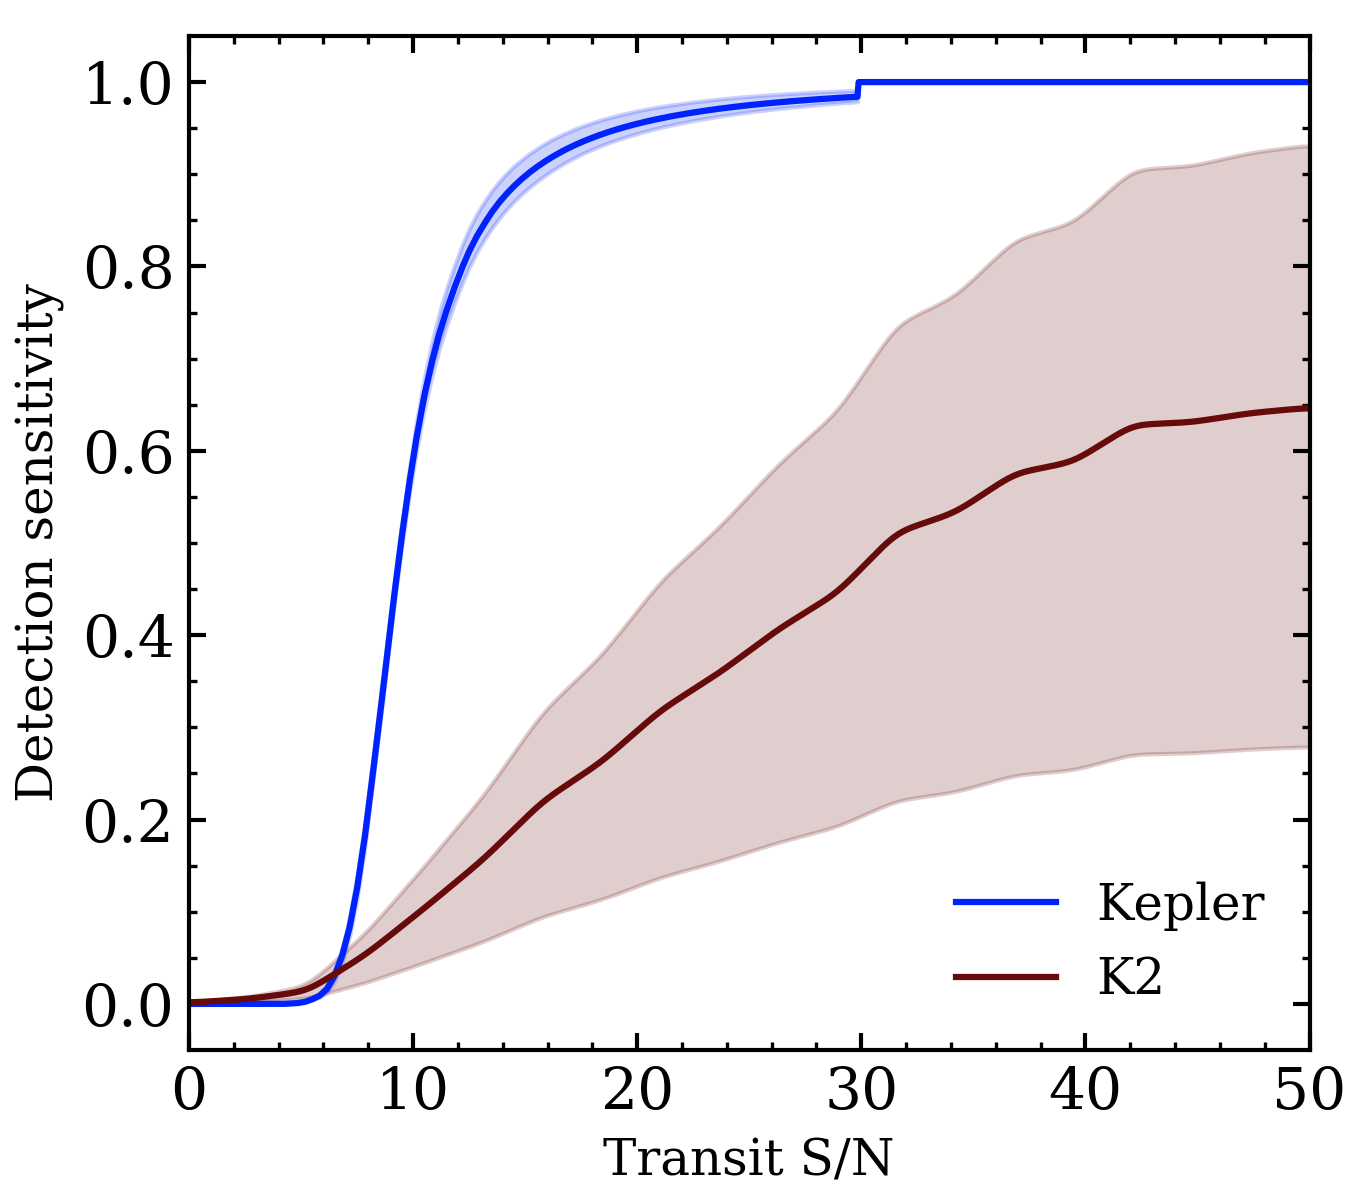
\includegraphics[width=0.98\hsize]{figures_tmp/senscurves.png}
  \caption{Average detection sensitivity for \kepler{} and \ktwo{.} The \emph{solid curves} represent the
    average transiting planet detection sensitivity for the \kepler{} and \ktwo{} stars in our sample as
    a function of the transit S/N (Eq.~\ref{eq:snr}). The shaded regions mark the 16$^{th}$ and 84$^{th}$
    percentiles of the measured detection sensitivities.} 
  \label{fig:senscurves}
\end{figure}


\subsection{K2 Sensitivity}
\texttt{EVEREST} light curves \citep{luger16,luger18}

as stated in Kruse+2019 section 4.1, \cite{luger16} find that everst outperforms k2sff and k2sc by $\sim 20-50$\% in terms of photometric precision

\texttt{ORION} \citep{cloutier19b}

\begin{figure*}
  \centering
  %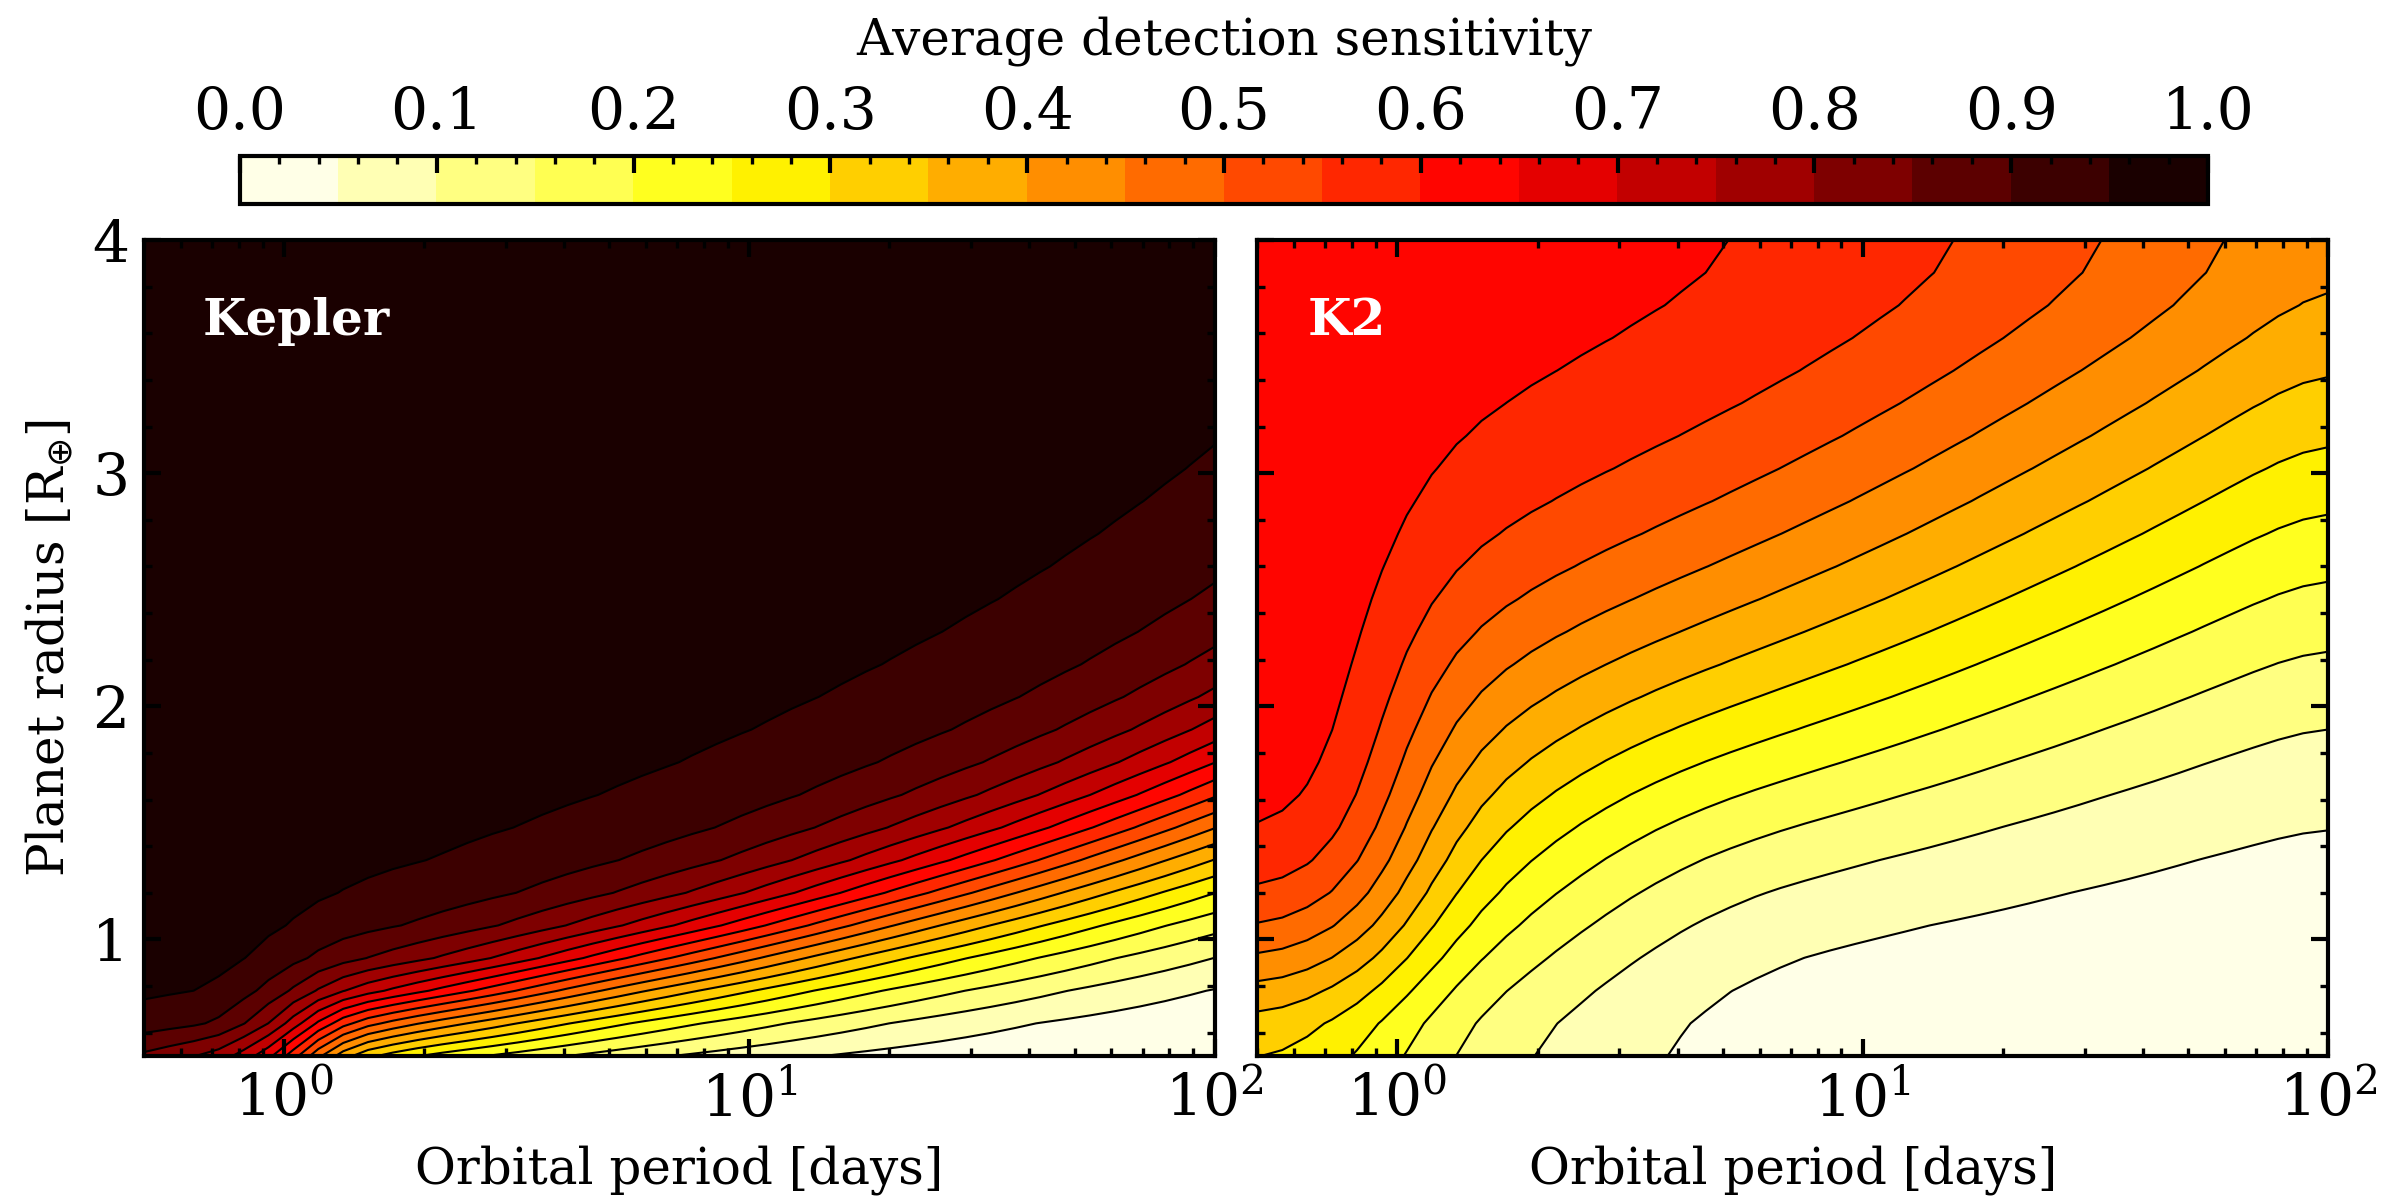
\includegraphics[width=0.98\hsize]{figures_tmp/sensmap.png}
  \caption{Average detection sensitivity and completeness versus orbital period and planetary radius.
    \emph{Top panels}: the average detection sensitivity for the \kepler{} and \ktwo{} stars in our stellar
    sample as functions of planetary radius and orbital period. \emph{Bottom panels}: the average completeness
    for the \kepler{} and \ktwo{} stars computed as the product of the detection sensitivity and transit
    probability (Eq.~\ref{eq:ptransit}).} 
  \label{fig:compmap}
\end{figure*}



\subsection{Survey Completeness}
Only transiting planets are detectable in transit surveys. To correct for the non-detection of otherwise
detectable but non-transiting planets around low mass stars in any \kepler{} or \ktwo{} field, we computed
the geometric transit probability for each star and at each grid cell $ij$ to be

\begin{equation}
  p_{t,nij} = \frac{R_{s,n} + r_{p,j}}{a_{ni}}. \label{eq:ptransit}
\end{equation}

\noindent Note that we are only interested in the relative occurrence rate and therefore do not consider
fixed scalar modifications to $p_{t,nij}$ for effects such as grazing transits or eccentricity corrections
\citep{barnes07b}.

Combining each star's detection sensitivity with the geometric transit probability yields our completeness
correction over the $ij$ grid. The average completeness maps for our \kepler{} and \ktwo{} stars are also
included in Fig.~\ref{fig:maps} as functions of $r_p$, $P$, and $F$.



\section{The Occurrence Rate of Small Close-in Planets around Low Mass Dwarf Stars} \label{sect:occurrence}
The detection and confirmation of planets from the \kepler{} and \ktwo{} surveys enable to measurement of the
occurrence rate of planets given the completeness corrections derived in Sect.~\ref{sect:completeness}.
For the indices $i$ and $j$ representing a planet's orbital period and radius, the probability of detecting
$k_{ij}$ such planets around the $N_s$ stars in our sample is given by the binomial distribution

\begin{equation}
  \mathcal{L}_{nij}(k_{ij}|N_s,p_{nij}) = \binom{N_s}{k_{ij}} \prod_{n=1}^{N_s} p_{nij}^{k_{ij}} (1-p_{nij})^{N_s-k_{ij}} 
%  \mathcal{L}_{nij}(k_{ij}|N_s,p_{nij}) = \frac{N_s}{k_{ij}} \prod_{n=1}^{N_s} p_{nij}^{k_{ij}} (1-p_{nij})^{N_s-k_{ij}} 
\end{equation}

\noindent where

\begin{equation}
  p_{nij} = f_{ij} \cdot s_{nij} \cdot p_{t,nij},
\end{equation}

\noindent is the probability of detecting a planet around the $n^{\text{th}}$ star and is dependent on the
intrinsic occurrence rate of planets $f_{ij}$, the detection sensitivity to such planets $s_{nij}$, the
the transit probability of such planets $p_{t,nij}$.




\begin{figure*}
  \centering
  %\includegraphics[width=.98\hsize]{figures_tmp/fmap.png}
  \caption{Planet occurrence rate versus orbital period and planetary radius.}
  \label{fig:fmap}
\end{figure*}
  
\begin{figure*}
  \centering
  %\includegraphics[width=.98\hsize]{figures_tmp/rphist.png}
  \caption{Occurrence rate of planets as a function of size. Histogram depicting the relative occurrence
    rate of close-in planets---with orbital periods $<100$ days---derived from the joint sample of confirmed
    planets from \kepler{} and \ktwo{} around low mass stars. The bimodal distribution of planet radii peaking
    at 1.15 and 2.0 R$_{\oplus}$ is resolved which highlights the presence of the radius valley at 1.6 R$_{\oplus}$.
    Uncertainties in the planet occurrences follow from binomial statistics and are limited by the relatively small
    number of confirmed planets around low mass stars from \kepler{} and \ktwo{.}}
  \label{fig:rphist}
\end{figure*}



\begin{figure*}
  \centering
  %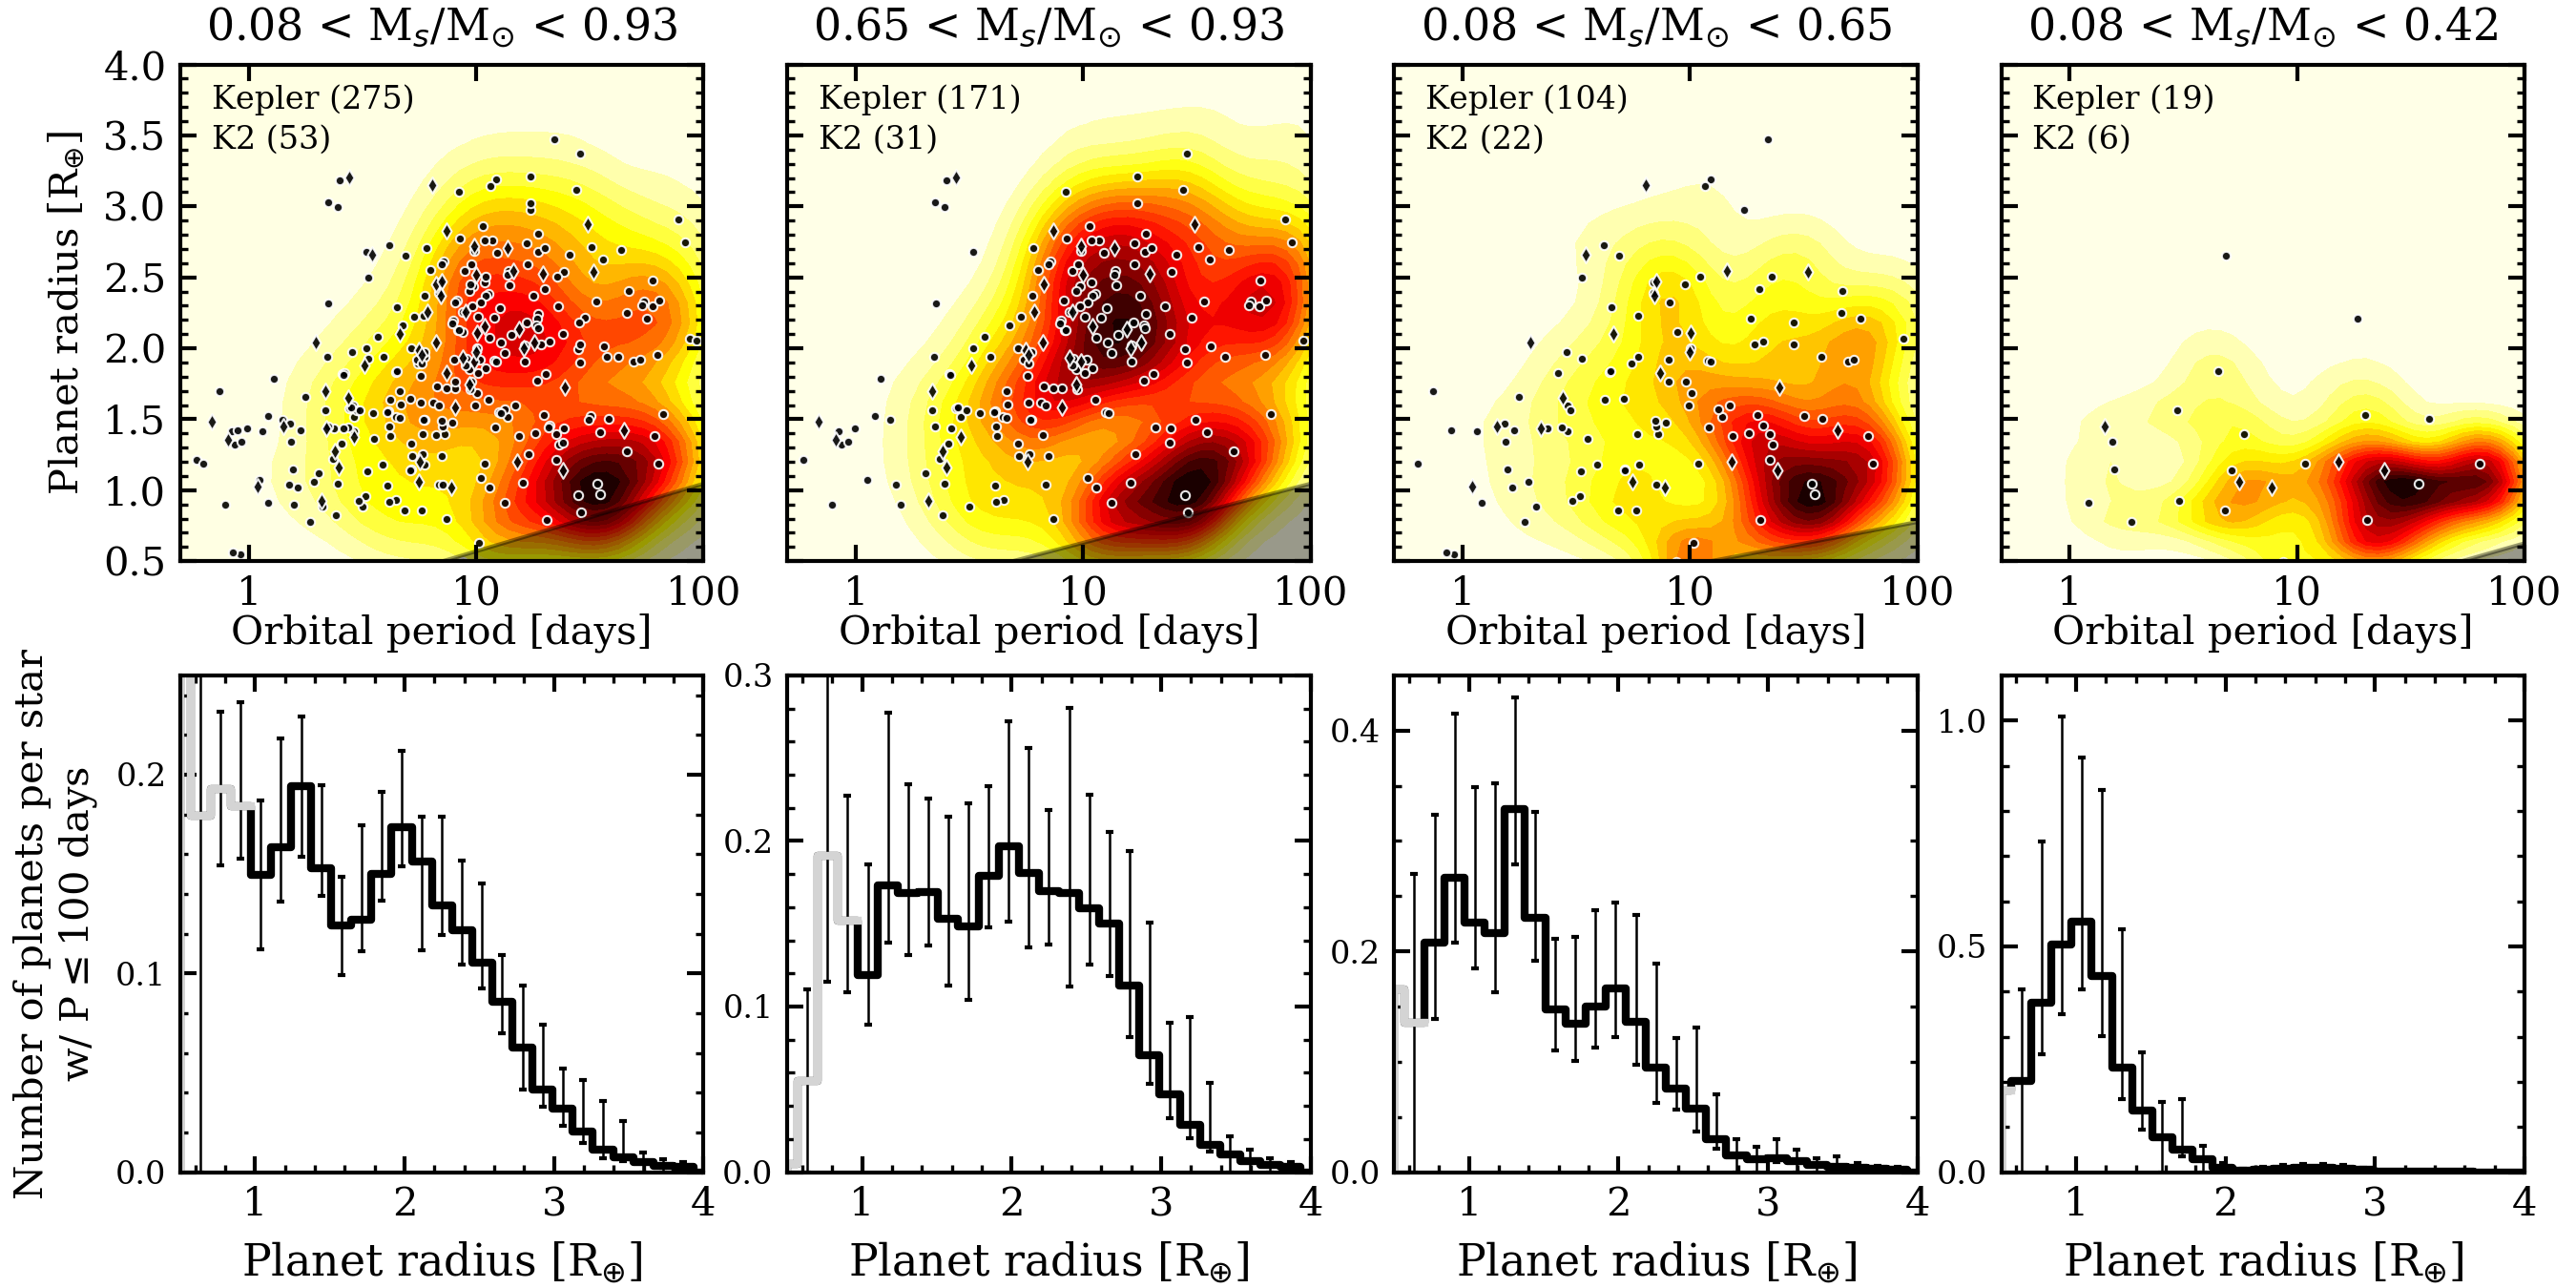
\includegraphics[width=.98\hsize]{figures_tmp/rphist_compMs.png}
  \caption{2D and 1D planet occurrence rates in various stellar mass bins. \emph{Top panels}: planet occurrence
    rate maps as a function of orbital period and planet radius. \emph{Bottom panels}: histograms of the relative
    planet occcurrence rate as a function of planet size. Each column corresponds to a unique cut in stellar masses
    representing the full stellar sample ($M_s \in [0,0.8]$ M$_{\odot}$), the early half ($M_s \in [0.63,0.8]$
    M$_{\odot}$), the late half ($M_s \in [0,0.63]$ M$_{\odot}$), and low mass cutoff ($M_s \in [0,0.42]$ M$_{\odot}$).
    As the stellar mass range is decreased the statistics become poorer which muddles the detection of the radius
    valley in any subset other than the full sample.} 
  \label{fig:rphistcomp}
\end{figure*}


\section{On the Physical Origin of the Radius Valley} \label{sect:models}

\begin{figure*}
  \centering
  %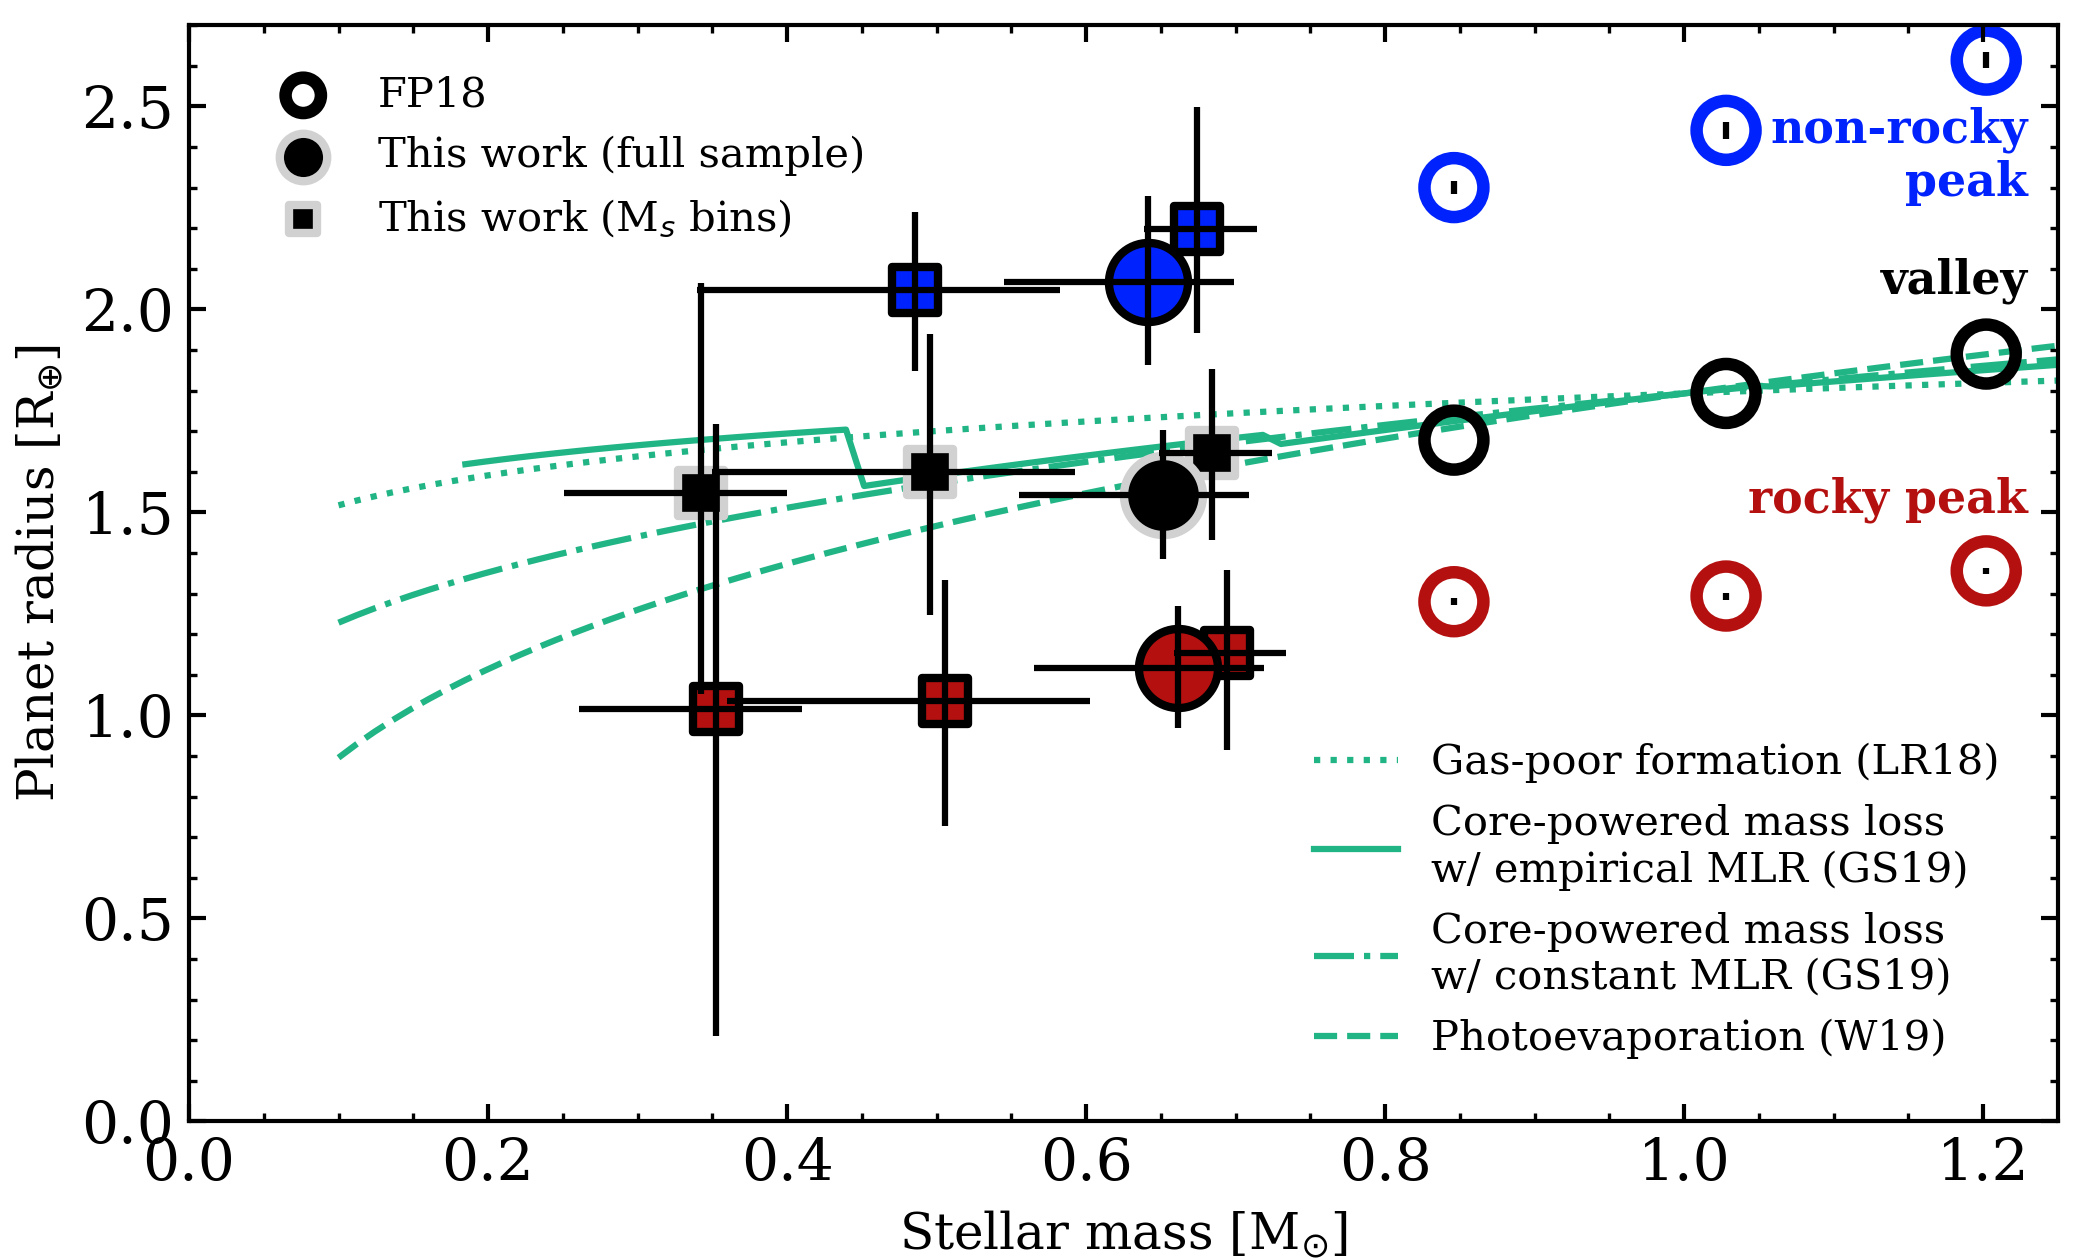
\includegraphics[width=0.98\hsize]{figures_tmp/rpvMsFULL_KepK2.png}
  \caption{Evolution of the radius valley with stellar mass. \emph{Solid markers}:
    the occurrence rate-weighted locations of the super-Earth peak (\emph{blue markers}), the
    radius valley (\emph{green markers}). and the sub-Neptune peak (\emph{red markers})
    as a function of host stellar mass for three $M_s$ bins considered in
    this work: $M_s \in [0,0.8]$ M$_{\odot}$, $M_s \in [0,0.8]$ M$_{\odot}$, and $M_s \in [0,0.8]$ M$_{\odot}$. The median stellar masses
    are depicted along with their uncertainties calculated from the 16$^{th}$ and 84$^{th}$ percentiles their respective stellar
    mass distribution. Uncertainties on the
    peak and valley locations are derived by sampling the measured occurrence rates and their uncertainties along
    with samples of the hyperparameters controlling map smoothing, minimum detection sensitivity, and the assumed feature ranges in
    planet radius. Similar measurements for Sun-like stars from \cite{fulton18} are plotted as \emph{open markers}. The remaining
    curves represent theoretical predictions of the location of the radius valley based on models of atmospheric loss from
    core-powered luminosity with a constant mass-luminosity relation (\emph{dashed}; \citealt{gupta19b}), an empirical mass-luminosity
    relation (\emph{dotted}; \citealt{gupta19b}), and photoevaporation (\emph{solid}; \citealt{wu19}).
    The model curves are anchored at the valley location for $M_s = \text{M}_{\odot}$.}
  \label{fig:rpvMs}
\end{figure*}


\section{Improvements Afforded by TESS} \label{sect:tess}
NASA's Transiting Exoplanet Survey Satellite \citep[\tess{;}][]{ricker15} will provide hundreds of new transiting planet
dicsoveries in the vicinity of the radius valley \citep{barclay18}. \tess{} is particularly well-suited to the discovery of
close-in planets around low mass stars due to its red bandpass and its high cadence observations of $\sim 94$\% of the sky
following its first extended mission. 


given the TOIs that we have so far from TESS, reduced by the FP rate thus far, and scaled up to 1) the full TESS mission and 2) its extended mission, 
we can estimate the number of close-in M dwarf planets that are expected from TESS from the two aforementioned campaigns. from this we can add that 
planet population to those in this paper (maybe also add K2 candidates) and recalculate the position of the radius gap to improve its precision as 
a function of stellar mass. maybe we will be able to push down to lower mass stars

kk no better yet, lets compute the number of planets we need in different stellar mass bins to say something interesting about how the gap evolves 
with stellar mass. then using the calculation above, say how close to we come to doing that with TESS primary, TESS extended, TESS FFIs, and K2 
candidates.

\begin{figure}
  \centering
  %\includegraphics[width=0.98\hsize]{figures_tmp/rpuncertainty_TESS.png}
  \caption{Expected improvement in the measurement precision of the radius peak and valley locations with additional
    confirmed planets around stars with $M_s\sim 0.3$ M$_{\odot}$. Assuming a fixed detection probability (\textbf{dont do this}),
    the shaded
    regions depict the degree of improvement in the upper and lower limits on location of the super-Earth peak
    (\emph{blue}), the radius valley (\emph{green}), and the sub-Neptune peak (\emph{red}) as additional planets are
    detected by missions like TESS. For stars with $M_s\sim 0.3$ M$_{\odot}$, model predictions of the valley location
    from photoevaporation and core-powered mass loss differ by $\sim 0.4$ R$_{\oplus}$ (\emph{dashed horinzontal line}).
    Based on the performance of TESS to-date, the expected time to confirm such planets is parameterized as a linear
    function of time and is depicted on the secondary x-axis.}
  \label{fig:improve}
\end{figure}

\section{Discussion \& Conclusions} \label{sect:conclusion}
Many new and up-coming RV spectrographs (e.g. HARPS; \citealt{mayor03}, HIRES; \citealt{}, 
HARPS-N; \citealt{}, APF; \citealt{}, PFS; \citealt{}, NEID; \citealt{},
ESPRESSO; \citealt{}, SPIRou; \citealt{}, NIRPS; \citealt{},  HPF; \citealt{}, IRD; \citealt{},
Minerva-Australis; \citealt{})
will be partially focused on characterizing the masses of planets spanning the radius valley in order to
improve our physical understanding of the nature of those planets. The subset of those spectrographs operating
in the near-IR in particular will focus on M dwarf planetary systems. This work elucidates the location of
the radius valley around M dwarf host stars and guides observers to the planetary radii from transit surveys
that are of interest for fully characterizing the radius valley in terms of planetary bulk densities.

mass dependence of the gap: 

The weighted feature radii are also effected by planetary magnetic fields which directly impact the 
efficiency of atmospheric stripping in the photoevaportation scenario \citep{owen19}. The persistence 
of a planetary magnetic field acts to shield the planet's atmosphere from XUV stellar photons thus 
enhancing the retention of the atmosphere and shifting the location of the radius valley to larger 
radii.

In the photoevaporation scenario, the
partial filling of the gap around low mass stars may be explained by their lower XUV luminosities relative to 
Sun-like such as those included in the CKS stellar sample \citep{}.

This explanation seems to be supported by the stellar mass dependent gap measurements from \cite{fulton18}. 

summary of McDonald+2019 (https://ui-adsabs-harvard-edu.ezp-prod1.hul.harvard.edu/abs/2019ApJ...876...22M/abstract):
X-rays only since XUV observations are difficult for non-Sun-like stars and X-rays are the dominant driver of 
atmospheric loss by photoevaporation. 
Jackson+12 \& Shkolnik+14 derived scalings from data for the LX/Lbol evolution over time for 0.3 - 1.3 solar mass stars
on the MS, low mass stars ($\lesssim 0.8$ M$_{\odot}$) exhibit a LX/Lbol that is typically a few to ten times greater 
than around Sun-like stars ($0.8-1.12$ M$_{\odot}$) (fig 1 in McDonald+2019).
scaling these values by the typical bolometric luminosities of stars in the various mass bins reveals that 
Sun-like stars having higher absolute X-ray luminosities which contributes to more efficient clearing of the 
gap by photoevaporation.


\section{Methods}
%\textbf{maybe take the stance that we should only be using confirmed planets from either Kepler or K2. Although we
%know that the methods by which K2 planet candidates become confirmed is different and more time consuming than Kepler
%PCs, maybe we should just present that fact and say that we know  that many K2 PCs will turn out to be real planets
%but we don't know which ones yet. Because we have such a large sample of low mass K2 stars and so confirmed few
%planets, let's not try to derive the occurrence rate verbatim from K2 (because it's way off), but instead just
%scale the K2 cumulative occurrence over the parameter space of interest to what we get from Kepler, and then compare the two.}

The goal of this study is to extend measurements of the radius valley and its properties to planetary systems
hosted by low mass dwarf stars later than K3.5V \citep{pecaut13} with effective temperatures \teff{} $<4700$ K:
the lower limit of \teff{} considered by the California Kepler Survey where the radius valley was first revealed
\cite{fulton17}.
%\subsection{Kepler Stellar Sample} \label{sect:kep}
Our sample of \kepler{} stars is drawn from the cross-matched list of \kepler{} targets with the \gaia{} DR2
\citep{berger18} which reports stellar parallaxes, 2MASS $K_s$-band apparent magnitudes, and spectroscopic
measurements of \teff{,} \logg{,} and [Fe/H] for $\sim 178,000$ \kepler{} stars.
%Spectroscopic measurements were obtained from either the DR25
%Kepler Stellar Properties Catalog \citep[KSPC;][]{mathur17}, the California
%Kepler Survey \citep[CKS;][]{petigura17} where available, and \teff{} values for stars with \teff{} $<4000$ K were compiled from \cite{gaidos16}.
The stellar parameters were applied to the spectral classification code \texttt{isoclassify} \citep{huber17} to
calculate the stellar luminosities and consequently refine the stellar radii using the Stefan-Boltzmann law for
FGK \kepler{} stars. 
%\cite{berger18} applied the full set of available stellar parameters to the spectral classification code
%\texttt{isoclassify} \citep{huber17} to calculate stellar luminosities. The resulting luminosity values were
%consequently combined with the \teff{} measurements to refine the stellar radii using the Stefan-Boltzmann law
%for the majority of FGK \kepler{} stars.
However, bolometric corrections for M dwarfs with \teff{} $<4100$ K
%and absolute $K_s$-band magnitudes $M_{K_s}>3$
are known to suffer significant inaccuracies owing to incomplete molecular line lists. The stellar radii for
these stars are instead refined using empirically-derived M dwarf radius-luminosity relations \citep{mann15}.
%\cite{berger18} instead adopted the empirically-derived M dwarf radius-luminosity
%relation from \cite{mann15} to refine their M dwarf stellar radii. \cite{berger18} also used the \teff{} values and their
Effective temperatures and measured luminosities were also used to derive stellar evolutionary flags that enable
us to reject sub and red giants from our \kepler{} sample.
%Stellar masses $M_s$ are not reported by \cite{berger18}. In order to study the \kepler{} planet population as
%a fuction of $M_s$,
Stellar mass values are derived from the stellar radii using mass-radius relations applicable to K and M dwarfs
\citep{boyajian12}.
%\cite{boyajian12} acquired interferometric measurements with the CHARA array of 21 nearby K and M dwarfs
%to measure the angular size of each stellar disk at the level of $\lesssim 5$\%. Their stellar sample was supplemented by 12
%literature measurements of $R_s$ from interferometry. Mass measurements were then derived using the $K_S$-band mass-luminosity
%relation from \cite{henry93} which was valid for their full stellar sample spanning 0.13-0.9 R$_{\odot}$. \cite{boyajian12}
%The stellar mass-radius relation is parameterized as a quadratic in $M_s$ and reported value and uncertainties for each polynomial
%coefficient. Here, we assume independent Gaussian probability density functions (PDF) for each coefficient and sample their values
%along with each star's $R_s$ from its measurement uncertainty to derive stellar masses and uncertainities for all of the stars in
%our sample of low mass dwarfs.

%We define our final \kepler{} stellar sample by focusing on stars that statisfy the following
%criteria:

%\begin{enumerate}
%\item $T_{\text{eff}} - \sigma_{T_{\text{eff}}} \leq 4700$ K,
%\item $R_s - \sigma_{R_s} \leq 0.8$ R$_{\odot}$,
%\item $M_s - \sigma_{M_s} \leq 0.8$ M$_{\odot}$, and
%\item and an evolutionary flag corresponding to a dwarf star. 
%\end{enumerate}

%\noindent %That is that, we only consider dwarf stars that are consistent with being cooler than 4700 K, are smaller than
%%0.8 R$_{\odot}$, and are less massive than 0.8 M$_{\odot}$.
%Based on these criteria we retrieve \textbf{4241} low mass \kepler{} stars that are relevant to our study.
%The distributions of stellar parameters are depicted in Fig.~\ref{fig:stars}.
%The stars in this sample exhibit a median fractional radius uncertainty of $\sim \mathbf{7}$\% or about 4-5
%times smaller than the typical radius uncertainty reported in the KSPC. 


%\subsection{K2 Stellar Sample}
Our \ktwo{} stellar sample was compiled by first retrieving the list of probable low mass dwarf stars
from the Ecliptic Plane Input Catalog (EPIC) available on MAST\footnote{Mikulski Archive for Space Telescopes,
  \url{https://archive.stsci.edu/k2/}.} and using conservative restrictions on the assumed stellar parameters
of interest. 
%We first retrieved the list of probable low mass dwarf stars observed in any \ktwo{} campaign by querying
%MAST\footnote{Mikulski Archive for Space Telescopes, \url{https://archive.stsci.edu/k2/}.}. Our initial
%search was restricted to \ktwo{} stars with \teff{} $<4900$ K, \logg{} $>4$, and $R_s<1$ R$_{\odot}$. Note that these
%criteria are not intended to represent the parameter ranges for low mass dwarf stars but are intended as
%conservative conditions to encapsulate all such stars prior to their refinement based on the \gaia{} DR2
%data.
We search was limited to stars with \kepler{}
magnitude $K_p<\mathbf{15.55}$: the dimmest probable low mass star with a confirmed transiting planet from \ktwo{}
\citep[NASA Exoplanet Archive;][]{akeson13}. %From MAST we retrieve each star's Ecliptic Plane Input Catalog
%(EPIC) numerical identifier, stellar photometry in the \kepler{} bandpass $K_p$ and 2MASS bands $JHK_s$, along
%with measured values of \teff{,} \logg{,} [Fe/H], $R_s$, and $M_s$.
The stellar parameters are refined by cross-matching our initial \ktwo{} sample with \gaia{}  
DR2 using the \gaia{-}\ktwo{} data products from Megan Bedell\footnote{\url{https://gaia-kepler.fun/}}. %Using
%the EPIC identifiers we retrieve the celestial coordinates, stellar parallaxes $\varpi$, and \gaia{} photometry
%for stars in our preliminary \ktwo{} sample where available.
\ktwo{} stars that lack \gaia{} measurements are omitted from our sample.
Stellar radius measurements follow from the methodology applied to the \kepler{} stars 
%outlined in \cite{berger18}.
wherein stellar parallaxes are transformed to distances\citep{bailerjones18} which are then used along with
the source's celestial coordinates to interpolate the dust extinction maps using \texttt{mwdust} \citep{bovy16}
to derive extinction coefficients. 
%We use the formalism of \cite{bailerjones18} to transform the assumed
%Gaussian distributed $\varpi$ posteriors into stellar distance posteriors which need not remain Gaussian distributed.
%Using the measured distances $d$, 
%uncertainties, and celestial coordinates, we interpolate over the $E_{B-V}$ extinction maps using the
%\texttt{mwdust} software \citep{bovy16} to derive both the the $V$ and $K_s$-band extinction coefficients $A_V$ and
%$A_{K_s}$. From this we calculate each star's absolute $K_s$-band magnitude $M_{K_s} = K_s - \mu - A_{K_s}$ where
%the distance modulus is $\mu = 5\log_{10}(d/10\text{ pc})$.
For the earliest stars in our sample ($M_{K_s}\leq 4.6$) for which the bolometric corrections
are still reliable, we interpolate the MIST bolometric correction grids \citep{choi16} over \teff{,} \logg{,} [Fe/H],
and $A_V$ to derive the $K_s$-band bolometric corrections $BC_{K_s}$. At this point we compute the stellar bolometric
luminosity via

\begin{equation}
  L_{\text{bol}} = 3.0128 \times 10^{28} \text{W } 10^{-0.4 M_{\text{bol}}},
\end{equation}

\noindent where $M_{\text{bol}}=M_{K_s} + BC_{K_s}$ is the absolute bolometric magnitude. The refined stellar radii
are then calculated using the Stefan-Boltzmann law given $L_{\text{bol}}$ and \teff{} with measurement uncertainties
propagated throughout.

For the remaining late type stars with $M_{K_s}>4.6$ we revert to the empirically-derived radius-luminosity relation
from \cite{mann15} to calculate the M dwarf stellar radii. \cite{mann15} fit a second-order polynomial to $R_s$ as
a function of $M_{K_s}$ which has a characteristic dispersion in the fractional radius uncertainty of 2.89\%. To quantify
the final $R_s$ uncertainty we sample $M_{K_s}$ from its posterior PDF and transform each $M_{K_s}$ draw to an $R_s$ value
using the aforementioned radius-luminosity relation. To each star's dericed $R_s$ PDF, we add in quadrature an additional
dispersion term whose fractional radius uncertainty is 2.89\%.

Given the refined stellar radii for our \ktwo{} sample, we proceed with deriving stellar masses identically to the method
applied to the \kepler{} sample (see Sect.~\ref{sect:kep}) using the \cite{boyajian12} stellar mass-radius relation. 

We define our final \ktwo{} stellar sample of low mass dwarf stars similarly to our definition of the \kepler{} sample.
Explicitly, we focus on stars that obey the following criteria:

\begin{enumerate}
\item $T_{\text{eff}} - \sigma_{T_{\text{eff}}} \leq 4700$ K,
\item $R_s - \sigma_{R_s} \leq 0.8$ R$_{\odot}$,
\item $M_s - \sigma_{M_s} \leq 0.8$ M$_{\odot}$, and
\item $R_s > R_{s,\text{max}}$.
\end{enumerate}

\noindent Because our \ktwo{} sample lacks any evolutionary flags, we adopt the following ad hoc upper limit on $R_s$
from \cite{fulton18} that aims to reject evolved stars:

\begin{equation}
  R_{s,\text{max}} = \text{R}_{\odot} 10^{0.00025(T_{\text{eff}}/\text{K}-5000)+0.2}.
\end{equation}

\noindent Based on these criteria we retrieve \textbf{13565} low mass \ktwo{} stars that are relevant to our study.
The distribution of \ktwo{} stellar parameters are depicted in Fig.~\ref{fig:stars}.
The stars in this sample exhibit a median fractional radius uncertainty of $\sim \mathbf{4}$\%.

\begin{figure*}
  \centering
  %\includegraphics[width=0.49\hsize]{figures_tmp/stellar_corner_Kep.png}
  %\includegraphics[width=0.49\hsize]{figures_tmp/stellar_corner_K2.png}
  \caption{Stellar samples from \kepler{} and \ktwo{.} Distributions of Kepler magnitudes, effective temperatures,
    stellar radii, and stellar masses for stars in our final stellar sample from either \kepler{} (\emph{left panels})
    or \ktwo{} (\emph{right panels}).}
  \label{fig:stars}
\end{figure*}

\capstartfalse
\begin{deluxetable}{lccc}
\tabletypesize{\small}
\tablecaption{\ktwo{} false positive rates for small planets around cool stars\label{tab:FP}}
\tablehead{Reference & $N_{\text{FP}}$ & $N_{\text{VP}}$ & FP rate [\%]}
\startdata
\cite{montet15}\tablenotemark{a} & 0 & 8 & $<30.7$ \\
\cite{crossfield16b} & 2 & 39 & $4.9^{+6.0}_{-1.4}$ \\
\cite{dressing17} & 2 & 34 & $5.6^{+6.4}_{-2.0}$ \\
\cite{hirano18}\tablenotemark{a} & 0 & 16 & $<19.5$ \\
\cite{livingston18a}\tablenotemark{a}  & 0 & 14 & $<21.0$ \\
\cite{mayo18}\tablenotemark{b} & 1 & 14 & $6.7^{+12.4}_{-2.0}$
\enddata
\tablecomments{Within each study we only consider PCs with $r_p <4$ R$_{\oplus}$ and orbiting cool stars with \teff{} $<4700$ K. FP: false positive. VP: validated planet.}
\tablenotetext{a}{These studies do not detect any FPs such that the reported FP rate upper limit is represented by its 95\% confidence interval.}
\tablenotetext{b}{\cite{mayo18} did not explicitly classify their non-validated planets as FPs so we define FPs within their sample as any PC whose false positive probability exceeds 10\%.}
\end{deluxetable}
\capstarttrue




\bibliography{refs}{}
\bibliographystyle{aasjournal}

\end{document}
